% ---------------------------------------------------------------------
% Journal article on the hardware property checking via software netlists.
%
%   - 14 pages maximum, including everything
%   - TCAD requires 30% new content.
%   - page charges apply
% ---------------------------------------------------------------------

% For final copy to IEEE
\documentclass[journal]{IEEEtran}

% For the initial submission
%\documentclass[journal,draftclsnofoot,onecolumn]{IEEEtran}

% ---------------------------------------------------------------------
% External packages - keep these minimal!
% ---------------------------------------------------------------------
\usepackage{listings}
\usepackage{import}

\usepackage{graphicx}
\usepackage{times}
\usepackage{array}
\usepackage{graphicx,wrapfig}
\usepackage{cite}
\usepackage{tikz}
\usepackage{amsthm}
\usepackage{caption}
\usepackage{multirow}
\usetikzlibrary{plotmarks}
\usepackage{pgfplotstable}
\usepackage{pgfplots}
\usepackage{amsfonts}
\usepackage{amssymb}
\usepackage{amsmath}
\usepackage{stmaryrd}
\usepackage{color}
\usepackage{epsfig}
\usepackage{wasysym} 
\usepackage{paralist}
\usepackage[algo2e,linesnumbered,ruled,lined]{algorithm2e}
\usepackage{hyperref}
\usepackage{dcolumn}
\newcolumntype{Y}{D..{5.2}}
\newcolumntype{R}{D..{2.2}}
\newcolumntype{"}{@{\hskip\tabcolsep\vrule width 1pt\hskip\tabcolsep}}
\makeatother

%\usepackage{mathptm}
%\usepackage{microtype}
%\usepackage{inconsolata}
%\usepackage[subnum]{cases}
%\usepackage{colortbl}
%\usepackage{booktabs}
%\usepackage{verbatim}
%\usepackage{comment}
%\usepackage{psfrag}
%\usepackage{subfigure}

\newcommand{\tool}[1]{\textsc{#1}\xspace}
\newcommand{\cbmcv}{\tool{cbmc 5.0}}
\newcommand{\symex}{\tool{path-symex}}
\newcommand{\ebmc}{\tool{ebmc}}
\newcommand{\hector}{\tool{hector}}
%\newcommand{\slec}{\tool{slec}}
\newcommand{\symexv}{\tool{path-symex 5.0}}
\newcommand{\ebmcv}{\tool{ebmc 4.2}}
%\newcommand{\hwcbmcv}{\tool{hw-cbmc 5.0}}
%\newcommand{\verifox}{\tool{verifox 0.5}}
%\newcommand{\acdcl}{\tool{acdcl}}
%\newcommand{\summarizer}{\tool{summarizer 1.0}}
%\newcommand{\v{2}c}{\tool{v2c 0.4}}
% \newcommand{\ABC}{\tool{ABC}}
\newcommand{\yosys}{Yosys 0.5}
\newcommand{\longversion}[1]{}

% Author comments to each other.
\def\comment#1{{\color{red}#1}}  % display comments/notes.

\newcommand{\Remote}[1]{}
%\newcommand{\mydef}[1]{\begin{definition}#1\end{definition}}
\theoremstyle{definition}
\newtheorem{definition}{Definition}
\newtheorem{example}{Example}
%\newtheorem{example}{Example}[section]
 
\newcommand{\rmcmt}[1]{{\color{magenta}{#1}}}%#1
\newcommand{\tmcmt}[1]{{\color{red}{#1}}}%#1

\lstdefinestyle{base}{
  language=C,
  emptylines=1,
  breaklines=true,
  escapeinside={(*}{*)},
  basicstyle=\ttfamily\color{black},
  moredelim=**[is][\color{magenta}]{~}{~},
  %moredelim=**[is][\color{red}]{@}{@},
  moredelim=**[is][\color{blue}]{'}{'}
}

\lstset{basicstyle=\ttfamily}

% ---------------------------------------------------------------------
% Use millimetres as unit of length, of course.
% ---------------------------------------------------------------------
\setlength{\unitlength}{1mm}

% ---------------------------------------------------------------------
% Any macros we define will ultimately go here. Only absolutely 
% essential macros to be used!
% ---------------------------------------------------------------------
%%% Standard text acronyms

\newcommand{\para}[1]{
	\subsubsection*{\textbf{#1}}}
 
%\noindent
%\textbf{#1~}}

\newcommand{\cnf}{\textsc{cnf}\xspace}
\newcommand{\sat}{\textsc{sat}\xspace}
\newcommand{\smt}{\textsc{smt}\xspace}
\newcommand{\dpll}{\textsc{dpll}\xspace}
\newcommand{\fpdpll}{\textsc{fdpll}\xspace}
\newcommand{\cfg}{\textsc{cfg}\xspace}
\newcommand{\cfgs}{\textsc{cfg}s\xspace}
\newcommand{\acfg}{\textsc{acfg}\xspace}
\newcommand{\smpp}{\textsc{smpp}\xspace}
\newcommand{\cegar}{\textsc{cegar}\xspace}
\newcommand{\cdfl}{\textsc{cdfl}\xspace}
\newcommand{\cdflitv}{\textsc{cdfl}$(\itvdom)$\xspace}
\newcommand{\cdcl}{\textsc{cdcl}\xspace}
\newcommand{\cbmc}{\textsc{cbmc}\xspace}
\newcommand{\bmc}{\textsc{bmc}\xspace}
\newcommand{\cdflalgo}{\textsc{\textsf{cdfl}}\xspace}
\newcommand{\ieeefp}{\textsc{\textsf{IEEE 754}}\xspace}


%%%%%%%%%%%%%%%%%%%%%%%%%%%%%%% 
%%% Mathematical Symbols %%%
%%%%%%%%%%%%%%%%%%%%%%%%%%%%%%% 

%%% Sets and functions

\newcommand{\powerset}[1]{\ensuremath{\wp(#1)}}
\newcommand{\set}[1]{\ensuremath{\left\{#1\right\}}}
\newcommand{\setneg}[1]{\overline{#1}}
\newcommand{\setsep}{\ensuremath{~|~}}
\newcommand{\tuple}[1]{\ensuremath{(#1)}}

\newcommand{\bnf}{\ensuremath{\mathrel{\mathop{::}}=}}
\newcommand{\bnfsep}{~\mid~}

\newcommand{\true}{\mathsf{true}}
\newcommand{\false}{\mathsf{false}}

%%% Lattices
\newcommand{\sle}{\ensuremath{\sqsubseteq}}
\newcommand{\sles}{\ensuremath{\sqsubset}}
\newcommand{\sge}{\ensuremath{\sqsupseteq}}
\newcommand{\sges}{\ensuremath{\sqsupset}}
\newcommand{\join}{\ensuremath{\sqcup}}
\newcommand{\bigjoin}{\ensuremath{\bigsqcup}}
\newcommand{\meet}{\ensuremath{\sqcap}}
\newcommand{\bigmeet}{\ensuremath{\bigsqcap}}


%%% Program model

\newcommand{\vars}{\mathit{Var}}
\newcommand{\cvars}{\mathit{CVar}}
\newcommand{\vals}{\mathit{Val}}
\newcommand{\exps}{\mathit{Exp}}
\newcommand{\expr}{\mathit{exp}}
\newcommand{\bexps}{\mathit{B\!Exp}}
\newcommand{\envs}{\mathit{Env}}
\newcommand{\env}{\varepsilon}
\newcommand{\aenv}{\hat{\varepsilon}}
\newcommand{\assg}{\ensuremath{\mathrel{\mathop:}=}}
\newcommand{\cond}[1]{\ensuremath{[#1]}}
\newcommand{\choice}[1]{\ensuremath{\mathit{choose}\{#1\}}}
\newcommand{\loopstmt}[1]{\ensuremath{\mathit{loop}\{#1\}}}
\newcommand{\nondetstmt}[1]{\ensuremath{\mathit{nondet}\{#1\}}}
\newcommand{\lfp}{\mathsf{lfp}}
\newcommand{\gfp}{\mathsf{gfp}}

\newcommand{\locs}{\mathit{Loc}}
\newcommand{\stmt}{\ensuremath{\mathit{stmt}}}
\newcommand{\err}{\ensuremath{\lightning}}
\newcommand{\init}{\ensuremath{\mathit{init}}}
\newcommand{\reach}{\mathit{Reach}}
\newcommand{\loopfree}{\mathit{Loop-Free}}

\newcommand{\badprog}{\ensuremath{\mathit{Err}}}
\newcommand{\progexec}{\ensuremath{\mathit{Exec}}}
\newcommand{\absbadprog}{\ensuremath{\hat{\mathit{Err}}}}
% \newcommand{\inv}{\ensuremath{\mathit{Inv}}}
\newcommand{\absinv}{\ensuremath{\hat{\mathit{Inv}}}}
\newcommand{\safe}{\ensuremath{\mathit{Safe}}}
\newcommand{\abssafe}{\ensuremath{\hat{\mathit{Safe}}}}

%%% Standard Abstract interpretation 
%%%
\newcommand{\aenvs}{\mathit{A\!Env}}
\newcommand{\post}{\mathit{post}}
\newcommand{\lpost}[1]{\mathit{post}_{#1}}
\newcommand{\abspost}{\mathit{\hat{post}}}
\newcommand{\abslpost}[1]{\mathit{\hat{post}}_{#1}}

\newcommand{\absuawp}{\mathit{\breve{wp}}}


%%% Fixedpoint-DPLL
%%%
\newcommand{\cvals}{\mathit{CVals}}
\newcommand{\avals}{\mathit{AVals}}

\newcommand{\val}{\mathit{v}}
\newcommand{\aval}{\hat{\mathit{v}}}
\newcommand{\sem}[2]{\ensuremath{\llbracket #1 \rrbracket_{#2}}}
\newcommand{\rsem}[3]{\ensuremath{\llbracket #1 \rrbracket_{#2}^{#3}}}
\newcommand{\asem}[2]{\ensuremath{\|#1 \|_{#2}}}

\newcommand{\comps}{\mathit{Comp}}
%%\newcommand{\ccomp}[1]{\tilde{#1}}
\newcommand{\ccomp}[1]{\mathord{\sim}{#1}}
\newcommand{\rest}{R}
\newcommand{\makerest}[1]{\mathit{res}(#1)}
\newcommand{\restrictions}{\mathit{Res}}
\newcommand{\lrestrictions}{\mathit{LRes}}
\newcommand{\restrict}[2]{\ensuremath{#1\mathord{\downharpoonright_{#2}}}}
\newcommand{\implabel}{\mathit{st}}
\newcommand{\gimplabel}{\mathit{stg}}

\newcommand{\decs}{\mathit{Dec}}
\newcommand{\dec}{\mathsf{d}}
\newcommand{\imp}{\mathsf{i}}
\newcommand{\emptystack}{\epsilon}

\newcommand{\lit}{\ell}
\newcommand{\lits}{\mathit{Lit}}
\newcommand{\litseq}{L}
\newcommand{\stackres}[1]{\lfloor #1\rfloor}
\newcommand{\litrest}[1]{\langle#1\rangle}
\newcommand{\litres}{\mathit{lit}}

\newcommand{\solver}[2]{#1 ~\|~ #2}

%%% Pseudocode
\newcommand{\pdeduce}{\mathsf{deduce}}
\newcommand{\pdecide}{\mathsf{decide}}
\newcommand{\pmaximal}{\mathsf{maximal}}
\newcommand{\plearn}{\mathsf{learn}}
\newcommand{\pbacktrack}{\mathsf{backtrack}}
\newcommand{\pfail}{\mathsf{fail}}
\newcommand{\psafe}{\mathsf{safe}}

 \newcommand{\fpfont}[1]{\textbf{\sffamily{#1}}}
 \newcommand{\fpfn}[1]{\sffamily{#1}}
 \SetKwSty{fpfont}
 \SetFuncSty{fpfn}

 \SetKwFunction{Decide}{decide}
 \SetKwFunction{TransProp}{tprop}
 \SetKwFunction{UnitProp}{uprop}
 \SetKwFunction{Refines}{refines}
 \SetKwFunction{Deduce}{deduce}
 \SetKwFunction{IsUnit}{is\_unit}
 \SetKwFunction{Propagate}{propagate}
 \SetKwFunction{Invariant}{invariant}
 \SetKwFunction{Atomic}{atomic}
 \SetKwFunction{Learn}{learn}
 \SetKwFunction{Backtrack}{backtrack}
 \SetKwFunction{Clausegen}{clauseGen}
 \SetKwFunction{Invariantgen}{invariantGen}

 \SetKw{Let}{let}

%%% Generalization
\SetKwFunction{Asserting}{asserting}
\SetKwFunction{Cutheur}{cutheur}
\SetKwFunction{Generalise}{generalise}
\SetKwFunction{Analyse}{analyse}
\SetKwFunction{ClauseGeneralise}{clauseGeneralise}
\SetKwFunction{WpGeneralise}{wpGeneralise}
\SetKw{MyCase}{case}
\SetKwFunction{SetReason}{setReason}
\SetKwFunction{PickAssertingCut}{assertingCut}
\newcommand{\reasons}{\mathit{Reasons}}
\newcommand{\implicationgraph}{\mathit{implicationGraph}}

%%% Operators
\newcommand{\wrt}{w.r.t.\ }
% \newcommand{\inp}{\mathit{input}}
\newcommand{\M}{{\cal M}}
\newcommand{\Tr}{{\mathit{tr}}}
\newcommand{\clip}{{\mathit{clip}}}
\newcommand{\decomp}{{\mathit{decomp}}}
\newcommand{\form}{{\mathit{Form}}}
\newcommand{\clausecompl}{\mathit{clcomp}}
\newcommand{\covers}{{\mathit{covers}}}
\newcommand{\cfgdecomps}{{\cal D}_{\mathit{CFG}}}
\newcommand{\cfgrefine}{{\cal R}_{\mathit{CFG}}}
\newcommand{\literals}{{\cal L}}
\newcommand{\clauses}{{\cal C}}
\newcommand{\proofstate}{\mathit{proof}}
\newcommand{\literaldecomp}[1]{\mathit{lits(}#1\mathit{)}}
\newcommand{\transded}{\mathit{trans}}
\newcommand{\unitded}{\mathit{unit}}

\newcommand{\prog}{P}

\newcommand{\intervals}{\mathit{Itv}}
\renewcommand{\min}{\mathit{min}}
\renewcommand{\max}{\mathit{max}}
\newcommand{\itvdom}{{\mathit{IEnv}}}
\newcommand{\atoms}{\mathit{Atoms}}

\newcommand{\irred}{\mathit{Irred}_\meet}

\newcommand{\implsu}{I_\mathsf{u}}
\newcommand{\implst}{I_\mathsf{t}}

\newcommand{\predec}{\mathit{predec}}
\newcommand{\conflictnode}{\mathit{conflict}}

\newcommand{\dred}[1]{\textcolor{red!60!black}{#1}}
\newcommand{\dgreen}[1]{\textcolor{green!40!black}{#1}}



% ---------------------------------------------------------------------
% Start of document
% ---------------------------------------------------------------------
\begin{document}

% ---------------------------------------------------------------------
% Title, authors, abstract, keywords
% ---------------------------------------------------------------------
\title{Exploring Formal Verification of Hardware Properties using Software Analysis Tools}

\author{Rajdeep Mukherjee, 
        Peter Schrammel,
        Daniel Kroening, 
        Tom Melham, \\
        Antoine Min{\'e} and
        Eugene Goldberg
        \thanks{R. Mukherjee, D. Kroening and T. Melham are at 
                University of Oxford, Department of Computer Science,
                Wolfson Building, Parks Road,
                Oxford, OX1 3QD, England.}
        \thanks{P. Schrammel is at  Diffblue Limited, Oxford, UK, and
                School of Engineering and Informatics,
                University of Sussex, Brighton, BN1 9RH, UK}
        \thanks{E. Goldberg is at Diffblue Limited, Oxford, UK}
        \thanks{A. Min{\'e} is at Engineering School, UPMC University, Paris}}
\markboth{IEEE Transactions on Computer-Aided Design of Integrated
          Circuits And Systems, Vol. XX, No. Y, Month 2004}%
         {Mukherjee et al.: Hardware Propety Verification using Software Analyzers}

% Create the title
\maketitle
% \IEEEpeerreviewmaketitle

\begin{abstract}
%
This paper explores formal verification of hardware via translation of
Verilog RTL into a novel ANSI-C representation called a \emph{software
netlist}.  Unlike abstract software models of hardware designed for
high-performance simulation, software netlists are cycle-accurate, faithful
translations of the RTL.  This precise representation enables novel
experiments with software verification technologies for formal verification
of hardware at the register-transfer level of abstraction.  To establish an
experimental baseline, we compare the capability and performance of native
tools for RTL and software verification tools that use propositional SAT/SMT
solvers for bit-level analysis.  We also evaluate some contemporary software
verification tools that use abstraction, such as classical abstract
interpretation and counterexample-guided abstraction refinement. 
Experiments with 34 RTL benchmarks confirm that SAT-based, bit-level
hardware model checkers currently outperform bit-level software analyzers. 
However, we also establish that abstract interpretation with manual guidance
is effective for finding complex bugs, as well as for proving unbounded safety
of software netlist designs generated from RTL circuits.
%
\end{abstract}

\begin{IEEEkeywords}
Formal verification, Verilog RTL, ANSI-C, SAT, Abstract Interpretation, 
Symbolic Execution.
\end{IEEEkeywords}

% ---------------------------------------------------------------------
% Start of text.
% ---------------------------------------------------------------------
\section{Introduction}\label{sec:intro}
%
Formal verification is now a well-established technology for in hardware design~\cite{Seligman:2015:FV}.  
From modest beginnings in the 1980s,
extensive corporate and academic research in hardware verification has gone
hand-in-hand with gradual but sustained industrial take-up.  Landmark
achievements in full correctness of commercial designs include the
verification of the entire execution clusters of the Intel Core 2
Duo~\cite{Core2} and Core i7 processors~\cite{i7} and the end-to-end ISA
verification of several ARM processors~\cite{ARM}.  The most prevalent
methodology, assertion-based verification~\cite{Foster:2009:AAB}, is now
well supported by mature tools supplied by electronics design automation (EDA) companies.

The industrial success of formal hardware verification has been enabled by
decades of research into specialised data structures and
algorithms~\cite{ic3, fmcad2000, ken, biere, STE},
tools~\cite{Seger:2005:IEE, abc, ebmc, vis, cadence, synopsysfv}, and
methodology~\cite{MCMILLAN2000279, Aagaard:2000:MLH, uclid, word-term,
word-bmc, DBLP:conf/lpar/AndrausLS08}.  The most widely used technology
relies on back-end analysis by propositional satisfiability (SAT)
solvers~\cite{Biere1999} or by modern solvers for satisfiability modulo
theories (SMT)~\cite{decision_procedures,
DBLP:conf/lpar/AndrausLS08,soc-keating,
DBLP:conf/mtv/SunkariCVM07,DBLP:conf/cav/Bjesse08}.  Scientifically inspired
and practically fruitful research into hardware verification continues
today, with scalability an ever-present challenge.

But the past two decades have also seen an explosion in research into
automated formal verfication of \emph{software}~\cite{dkw2008}, with
progress vivdly witnessed by the yearly `SV-COMP'
competition~\cite{Beyer2017}.  Verification of industrial-scale software is
now an established possibility, and commerial offerings are starting to
appear.  Some techniques used in software verification, such as
interpolation~\cite{Interpolants, Kroening:2011:ISV}, have analogues in
hardware verification.  Others, such as abstract
interpretation~\cite{CousotCousot77, Cousot:1996:AI}, have been largely
confined to the software domain.

In this paper, we explore the potential to leverage past and future progress
in automated software verification for hardware verification.  We~translate
a hardware model, articulated in Verilog at register transfer level (RTL),
into a \emph{software netlist}, an ANSI-C program that faithfully reproduces
the hardware in software.  This opens the door to experiments with software
verification technologies, arising from contemporary program analysis
research, to formal verification of hardware RTL designs.  We have two aims:
first, to establish baseline experimental data for verification of hardware
by translation into software; second, to evaluate the effectiveness of
software verification methods---notably abstract interpretation---that have
not yet been investigated for hardware.

Of course, the idea of expressing RTL designs in software has been
advocated in the past, primarily to enable faster simulation.  We mention
only~\cite{soc-keating}, which highlights verification-related benefits in
the context of SoC design.  But we emphasize that the software models
in~\cite{soc-keating} are abstractions of hardware that are usually written
manually and disconnected from the `golden' RTL design from which the chip
is ultimately realized.

By contrast, our software netlist representation is an exact
translation of the RTL design, not an abstract simulation model.  This is a
deliberate design choice, aiming to produce a faithful and transparent
software model that leaves maximum flexibility for software verification
proof strategies.  The principles behind the translation, which we have
implemented in a tool called V2C, are explained in Section~\ref{sec:v2c}.

Using our translation, we have experimentally investigated formal
verification of hardware using a range of native software analyzers.  For
baseline comparison with RTL verification tools, we experiment with software
verification technologies that employ SAT/SMT decision
procedures~\cite{DBLP:conf/cav/BeyerK11, 2ls, cbmc.tacas:2004,
DBLP:conf/tacas/HeizmannDGLMSP16}.  To probe the frontiers, we evaluate the
use of abstraction-based software verification techniques---most notably
abstract interpretation.  To ensure our results are openly accessible and
can be independently validated, our experiments compare the performance of
tools drawn from the Hardware Model Checking Competition
(HWMCC) against software verifiers from the Software Verification
Competition (SV-COMP).

Extensive experiments with 34 RTL benchmarks confirm that SAT-based,
bit-level hardware model checkers currently outperform bit-level software
analyzers.  But our experiments also show that a commercial abstract
interpreter, Astr{\'e}e, is---with manual guidance---particularly effective for
finding complex bugs, as well as for proving unbounded safety of software netlists.  
Unlike conventional SAT/SMT-based hardware verification, which
bit-blasts the design into propositional logic, abstract interpretation
analyzes the design over an abstract domain by computing a least fixed
point of the set of equations derived from the design.  Abstract
interpretation leverages the expressiveness of the underlying
numerical abstract domains for representing the relational and
non-relational invariants required for unbounded proofs or finding bugs.

Our experiments show that the performance of Astr{\'e}e is comparable to the
bit-level hardware model checker ABC~\cite{abc} and in some cases Astr{\'e}e
is faster for finding bugs.  It is worth noting that this technique does not
bit-blast the design, hence it is also more scalable than SAT/SMT-based
analysis.  However, abstract interpretation typically suffers from
imprecision due to the use of non-disjunctive abstract domains~\cite{nd}
that cannot precisely represent disjunctions.  Astr{\'e}e shows a high
degree of imprecision on our benchmarks.  We mitigate the imprecision by
manual trace partitioning, as explained in Section~\ref{abstraction}.

% ---------------------------------------------------------------------
% New Contributions Statement 
% ---------------------------------------------------------------------

Our previous work produced preliminary results 
for bounded and unbounded safety verification of RTL designs using 
software analyzers~\cite{mkm2015,mskm2016}.  
The results in these papers were restricted to a smaller set 
of benchmarks and fewer application of verification tools than we
explore here.  
The work presented here also makes significant technical contributions 
beyond those in~\cite{mkm2015,mskm2016} for formal 
verification of hardware RTL designs using state-of-the-art software analyzers 
based on SAT/SMT solvers as well as abstraction-based techniques. 
In particular, we present here a formal description of unbounded 
verification algorithms with a special emphasis on the application of  
classical abstract interpretation for precise safety verification.  In addition, 
this paper gives a more detailed analysis of a range of precise SAT/SMT-based 
and abstraction-based software verification tools for verifying a diverse set of 34 RTL 
circuits drawn from various sources.  We also present a notion of 
equivalence between a RTL and software netlist design for the purposes of RTL 
verification.  Finally, this paper reports on an experimental comparison of
bit-level and word-level verification using SAT and SMT solvers respectively. 

                   % Motivation, vision, and contributions
\section{Notation and Problem Statement}~\label{sec:notation}

A Boolean \textit{transition system} for bit-level hardware
modelling is a 3-tuple $T = \langle I,X,\delta \rangle$, where $X = \{x_1,\dots ,x_n\}$
is a finite set of \textit{state variables} ranging over the Booleans $\mathbb{B}$. 
Corresponding to the variables in $X$ is a set of primed \textit{next-state} variables  $X' = \{x_1', \dots, x_n'\}$.
A \textit{state} $s$ of $T$ is an assignment of Boolean values to the variables in $X$. Likewise, a \textit{next state} is an assignment of Boolean values to the variables in $X'$.  For any state $s$ that assigns values to the  variables $X$, we write $s'$ to denote the next state that assigns the same values to the corresponding primed variables in $X'$. If $F[X]$ is a formula over the variables $X$, we write $F(s)$ to say that
the assignment $s$ makes the formula $F[X]$ true. That is, the state $s$ satisfies $F$. Similarly, if $R[X,X']$ is a relation over the variables $X$ and $X'$, we write $R(s_1,s_2)$ to say that the state $s_1$ and the next state $s_2$ jointly satisfy the relation $R$. \tmcmt{Do we ever actually \textit{use} state notation?}

In a context in which a formula has been written $F[X]$, subsequent use of the notation $F[Y]$ for
some other set of variables $Y = \{y_1, \dots, y_n\}$ should be understood to mean the
result of substituting each variable in $Y$ for every occurrence of the corresponding variable in $X$ throughout the formula $F[X]$. Similarly, for $R[X,X']$ we may subsequently write $R[Y,Y']$, denoting the result of substituting variables in $Y$ and $Y'$ for corresponding variables in $X$ and $X'$.

In a transition system $T$, the predicate $I[X]$ is a formula over the variables in 
$X$ specifying the \textit{initial states} of the system; these are all the states 
$s$ for which $I(s)$. The formula $\delta[X,X']$ represents the \textit{transition relation} of the system; it stipulates the relationship that the system
realizes between current and next states at each discrete step of its operation.
Given a sequence of state variables $X_0, \dots, X_k$, the abbreviation \[ \delta_k = \underset{i \in [0,k-1]}{\bigwedge} \delta[X_i, X_{i+1}]\] 
will be used to denote $k$ steps of the transition system.
We call a sequence of states $(s_j,\dots,s_k)$ a~\textit{trace}
if $\delta(s_i,s'_{i{+}1})$ for $i=j,\dots,k-1$.  Such a trace is
said to be \textit{initialized} if $I(s_j)$.
  
A \textit{safety property} $P[X]$ is a predicate over the variables $X$ of $T$.  We will 
say a state $s$ is \textit{good} with respect to this property if $P(s)$; otherwise it is \textit{bad}. 
We will use the abbreviation \[P_k = \underset{i \in [0,k-1]}{\bigwedge} B[X_i]\]
in conjunction with $\delta_k$ to say that every trace of $k$ states are good.  Finally, a property $P$ is \textit{inductive} if $P[X] \wedge \delta[X,X']$ implies $P[X']$.    \tmcmt{Rajdeep - do we ever use the concept of `inductive'?}
\rmcmt{Yes, we use it later while explaining the various algorithms. Also, in the experimental results, where we find inductive invariants for some designs.}

\subsection{Problem Statement} 

We now define the \textit{safety verification} of a transition system~$T = \langle I,X,\delta\rangle$.
This is commonly known as the \textit{hardware model checking problem}.  
Given a safety property $P[X]$, the problem is to decide whether, starting from any initial state, a bad state can be reached following any sequence of transitions allowed by $\delta[X,X']$. In other words, is there an initialized trace of the system whose final state is bad?

                % Notation and definition of problem
\section{Background on Property Checking Methods}\label{sec:techniques}

In this section, we briefly sketch the verification methods for property checking that
we explore in our experiments. These are all well-established techniques and we refer 
the reader to the literature for more in-depth explanation.
For clarity, we give bit-level descriptions of these verification techniques, but
 many of them have analogues working at word-level.

We group techniques into two classes, based on whether 
they use bit-level decision procedures or employ abstract domains. We call these 
\textit{SAT/SMT-based Verification} and \textit{Abstraction-based Verification}, 
respectively.

\subsection{SAT/SMT-based Verification}~\label{netlist-verif}

The techniques in this class are all used for experiments with both conventional verification tools,
operating on RTL designs, and verification of  our software netlist representation using software analysis tools.

\para{Bounded Model Checking} 
%
BMC~\cite{biere} is a bug-finding method that searches for bad states along a finite trace of 
the transition system. Given a `depth' $k$ and a set of bad states characterised by a predicate
$B$, BMC forms the logical characterization of a $k$-length chain of transitions along the 
transition relation $T$,  starting from any initial state satisfying $I(X_0)$. 
Conjoined to this is a predicate saying that one or more of the states encountered 
is bad:
%
\[ I(X_0) \wedge \delta(X_0, X_1) \wedge \dots 
   \wedge \delta(X_{k{-}1}, X_k) \wedge (B(X_0) \vee \dots \vee B(X_k)) \]

\noindent This formula which is then checked for satisfiability using an efficient SAT procedure.
If found satisfiable, a bad state---a potential design bug---has been idenified.

%-------------------------------------------------------------------------------
\para{BMC with K-induction} 
%
BMC technique is incomplete, since it searches only a finite trace of the system. 
The method of $k$-induction~\cite{fmcad2000} addresses this as follows.
%
The base case of the $k$-induction is the simple BMC problem shown before. If the 
base case is unsatisfiable, then the 
induction step is checked using the formula 
shown below.  
%
\[ P(x_0) \wedge_{i=0}^{k-1} (\delta_i \wedge P_i) \implies P_k \]
%
Thus, $k$-induction assumes that $P$ holds 
over $k-1$ time steps to increase the 
likelihood that $P$ holds in $k$-th time step.
%
%-------------------------------------------------------------------------------
\para{Interpolation-based Model Checking} 
%
Interpolation-based model checking~\cite{cav03} 
computes a step-wise overapproximation of the reachable state-space,
$Q$, for a fixed unrolling $k$ of $T$, which is shown as
follows.
%
\[ Q \wedge_{i=0}^{k-1} (\delta_i \wedge P_i) \implies P_k \]
%
The value of $k$ is increased when the implication fails. This
progressively yields better overapproximation by 
generating an interpolant between the $i$-th 
overapproximation and $k$-step unrolling.
%which may be sufficient to prove the property $P$. 
Thus, the interpolation technique computes an abstraction 
of the postcondition with respect to the property $P$, 
by deriving interpolants from the failure of the
BMC problem.
%
Interpolation-based model checking is a complete method 
for reachability analysis of finite-state systems. 
%

%-------------------------------------------------------------------------------
\para{Predicate Abstraction with CEGAR}
%
This technique computes an abstract model $\hat{T}$ from the concrete model
$T$ using existential abstraction~\cite{cav97,cav2000}. 
%
Given a concrete state $x$ which is the 
valuation of all registers and a set of 
predicates, $Pred=\{\pi_{i} \ldots \pi_{k}\}$, 
an abstract state $b$ is obtained by applying 
an abstraction function $\alpha$, such that $b=\alpha(x)$.  
%
The abstract state $b$ is given by a vector 
of Boolean values of the predicates in $Pred$. 
%which is obtained by applying all the predicates 
%to the concrete state, 
%
Let $S$ be the set of concrete states in $T$. 
%
We define the abstract model given by, 
$\hat{T} = \langle \hat{I}, \pi, \hat{\delta} \rangle$.  
We define the components of $\hat{T}$ and property 
verification using predicate abstraction below. 
%
\begin{enumerate}
\item Transition Relation: $\hat{\delta} \mathrel{\hat{=}} \{(b,b') \mid \exists x,x' \in S: \delta(x,x') 
\wedge \alpha(x) = b \wedge \alpha(x') = b' \} $, $x=\{x_1 \ldots x_n\}, 
b=\{b_1 \ldots b_n\}, b_i=\pi_{i}(x) $, $\pi_i$ is the predicate on concrete variable $x_i$.

\item Initial State: $\hat{I}(b) \mathrel{\hat{=}} 
\exists x \in S: (\alpha(x) = b) \wedge I(x)$

\item Safety Property: $\hat{P}(b) \mathrel{\hat{=}} 
\forall x \in S: ((\alpha(x) = b) \implies P(x))$.  
Thus, if property $\hat{P}$ holds on all reachable states of the abstract model $\hat{T}$,
then $P$ also holds on all reachable state of concrete model $T$.
\end{enumerate}

%-------------------------------------------------------------------------------
\para{Property Directed Reachability} 
%
The property directed reachability~\cite{fmcad07} technique is briefly 
described as follows. 
%
Let $\alpha_1(x), \alpha_2(x),\ldots,\alpha_n(x)$ be a sequence of 
inductive assertions generated by the PDR algorithm such that 
$P$ is an invariant of $T$ if the following conditions hold.
\begin{enumerate}
 \item $I(x) \implies P$
 \item $\forall i, I(x) \implies \alpha_i(x)$
 \item $\forall i, {\overset{k}{\underset{i=1}{\wedge}}} 
	 (\alpha_i(x) \wedge P(x) \wedge \delta(x,x') \implies \alpha_k(x'))$,
 $\alpha_k$ is inductive relative to $\alpha_1, \alpha_2,\ldots,\alpha_{k-1}$,
 \item $\forall i, {\overset{n}{\underset{i=1}{\wedge}}} 
	(\alpha_i(x) \wedge P(x) \wedge \delta(x,x') \implies P(x'))$, 
 $P$ is inductive relative to the inductive invariants $\alpha_1,\alpha_2,\ldots,\alpha_n$, 
\end{enumerate}
%
The algorithm computes successive intermediate 
inductive assertions by removing the counterexamples-to-induction states in 
property-directed fashion.  Thus, the technique computes an overapproximation 
of the set of reachable states in successive steps until it finds an 
inductive strengthening assertion sufficient to prove the property. 
%
\subsection{Abstraction-based Verification}~\label{software-verif}
%
We now describe few well-known abstraction-based verification 
techniques that analyzes the transition system by computing an 
abstract pre-condition or abstract post-condition over a given 
abstract domain. Until now, the techniques described below 
are purely used in the context of software programs. In this paper, 
we employ these techniques for verifying the software netlist designs 
generated from the RTL. 
%-------------------------------------------------------------------------------
\para{Abstract Interpretation} 
%
Abstract Interpretation~\cite{Cousot92,CC79,DBLP:conf/emsoft/Cousot07},
is a theory of sound approximation of program semantics based on lattice 
structures. Static analysis using abstract interpretation is widely used 
to verify properties of safety-critical systems. 
%
In abstract interpretation, a given program is analyzed 
with respect to a given \textit{abstract domain} $\domain$.  
The technique computes an abstraction of the postcondition to derive an 
inductive invariant $AInv$.
%which includes the start state and is an 
%overapproximation of the set of reachable states.  
Elements of an abstract domain can be sets or conjuncts 
of formulae~\cite{DBLP:conf/vmcai/BrainDHGK13}.  
Given a transition system $T$, a set of formulas $A$ each of which is an 
element of $\domain$, and property $P$ as above, $AInv$ is computed as follows. 
%abstract interpretation can be described as follows. 
%
\begin{enumerate}
\item  $\exists AInv \in A. \forall x_0, x_1. (I(x_0) \implies AInv(x_0)) 
\wedge (AInv(x_0) \wedge \delta(x_0, x_1) \implies AInv(x_1))$, 
\item $\forall x. (AInv(x) \implies \neg{P(x)})$
\end{enumerate}
%
%where $A$ is the set of formulae each of which is the element of the 
%chosen abstract domain. The system is safe if there is no model. 
\Omit{
If an $AInv$ cannot the above conditions does not hold, the technique computes 
either a stronger invariant $AInv$ or choose a more expressive 
abstract domain to prove safety.
}
\Omit{
%-------------------------------------------------------------------------------
\para{Path-based symbolic execution}
%-------------------------------------------------------------------------------
%
Path-based symbolic execution is an well-known technique in program verification 
that is used for automatic test case generation~\cite{DBLP:conf/osdi/CadarDE08}.
Techniques based on precise forward symbolic 
execution~\cite{DBLP:conf/osdi/CadarDE08, King:1976:SEP:360248.360252}
executes a single path of a program at a time with symbolic inputs 
to generate symbolic expressions which are then conjoined with
the specification and are checked using a SAT/SMT solvers. 
The generated symbolic expression contains logical conjunction 
of the guards and assignments along that path.  This approach generates many 
SAT/SMT queries and may suffer from path explosion problem.

A similar technique is proposed for RTL in~\cite{star}. 
For sequential circuits, symbolic expressions contain path variables which 
are annotated by the time cycle to which it belongs. The 
work of~\cite{DBLP:journals/todaes/LiuV14} analyzes the 
feasibility of every path in the RTL program using a hybrid 
of concrete and symbolic execution and property based pruning.
}
%
%-------------------------------------------------------------------------------
\para{Automata based Trace Abstraction with Interpolants}
%-------------------------------------------------------------------------------
%
Automata-theoretic approaches to program verification~\cite{DBLP:conf/cav/KupfermanV00,
DBLP:books/sp/cstoday95/Vardi95,DBLP:conf/cav/HeizmannHP13} construct 
an automaton that represents a program together with its specification.
The negation of the specification is encoded via error locations in the automaton, 
that is, the error location is an accepting state.  The program satisfies the 
specification iff each trace accepted by the automaton is infeasible.
%
One of the automata-theoretic approaches for program verification 
is implemented in a tool called 
\textit{UltimateAutomizer}~\cite{DBLP:conf/tacas/HeizmannDGLMSP16}. 
The technique in~\cite{DBLP:conf/tacas/HeizmannDGLMSP16} decompose a 
program into sets of traces, and the decomposition is guided by proofs that 
are obtained for single traces. For correct programs, every non-empty set 
of error traces is an abstraction of the feasible error traces.  
%It obtains a proof for a single trace and trace abstraction generalizes 
%these proofs and combines them.  
Each iteration of the algorithm tries to obtain loop invariants for the path program
induced by the current counterexample.  This may be done through different techniques 
which can be applied iteratively. Each technique provides a set of Hoare triples that constitutes a proof of
safety for the current counterexample.
As soon as a technique yields loop invariants, the algorithm use these loop
invariants during the refinement and generalization step of trace abstraction.  If all the 
techniques have been exhausted and a loop invariant has not been obtained yet, the algorithm
use some or all (depending on the strategy) of the obtained hoare triples and 
refine or generalize with them.  Note that refinement reduces the number of error traces. 
              % Background on property checking methods
\section{Translating RTL to Software Netlists}\label{sec:v2c}
%  
Verilog and C have many operators in common, but  Verilog also has
additional hardware-oriented operators such as part-select, bit-select from vectors, concatenation,
and reduction. Additionally, many Verilog statements have no direct analogue in C. Examples include
initial blocks, always blocks, generate statements, procedural assignments
(blocking, non-blocking) and continuous assignments. Verilog also supports the 4-valued data types
reg, wire, and integer.  All these constructs, combined with
parallelism, make translation challenging.

In view of these complexities, our translation is deliberately direct and transparent: we try to
preserve the structure of the RTL and refrain from optimizations or abstractions. Fidelity of the
resulting C code to the semantics of the original Verilog is prioritised---meaning that we rely on
the downstream software analysis tools for efficiency, rather than obscure our translation with
optimisations.

Verilog and C have many operators in common, but  Verilog also has 
additional hardware-oriented operators such as part-select, bit-select from vectors, concatenation, and reduction. Additionally, many Verilog statements have no direct analogue in C. Examples include
initial blocks, always blocks, generate statements, procedural assignments
(blocking, non-blocking) and continuous assignments. Verilog also supports the 4-valued data types 
reg, wire, and integer.  All these constructs, combined with 
parallelism, make translation challenging.

In view of these complexities, our translation is deliberately direct and transparent: we try to preserve the structure of the RTL and refrain from optimizations or abstractions. Fidelity of the resulting C code to the semantics of the original Verilog is prioritised---meaning that we rely on the downstream software analysis tools for efficiency, rather than obscure our translation with optimisations. 

\rmcmt{ EXAMPLE CHANGED, SEE SECTION 4}
Fig.~\ref{ex1} shows an illustrative example. \tmcmt{Rajdeep, please provide a couple of sentences of commentary to explain the example. Also, is this example going to be confusing because the `always' part is not translated?}
%
\Omit{
\begin{figure*}[t]
\scriptsize  
\centering
%\begin{tabular}{|l|l|l|l|}
\begin{tabular}{|l|l|l|}
\hline
%  Verilog & Formal Semantics & Synthesized Hardware & Software netlist \\
\textbf{Verilog} & \textbf{Synthesized Hardware} & \textbf{Software Netlist} \\
\hline
\begin{lstlisting}[mathescape=true,language=Verilog]
module top(clk, a);
input clk, a;
reg b,d,e; 
wire c,cond;
assign c = e ? 1'b0:d;
assign cond = a;
always @(posedge clk) 
 begin
  b<=a;
  if(cond && b)
   e<=b;
  else 
   e<=0;
  d<=c;
 end
endmodule
\end{lstlisting}
&
\begin{minipage}{4.0cm}
\centering
\scalebox{.5}{\import{figures/}{ckt.pspdftex}}
\end{minipage}
&
\begin{lstlisting}[mathescape=true,language=C]
struct state_elements_top {
 unsigned int b, d, e; };
struct state_elements_top  u1;
void top(_Bool clk, unsigned a) {
  _Bool c,cond;
  _Bool b_old=u1.b;
  cond = a;
  c = (u1.e)?0:u1.d;
  u1.b = a;
  if(cond && b_old)
    u1.e = b_old;
  else
    u1.e = 0;
  u1.d = c;  
}
\end{lstlisting}\\
\hline
\end{tabular}
\caption{Example of Verilog Translated into C}
\label{ex1}
\end{figure*}}

\subsection{Translation Flow and Software Netlist Structure}

Our translation is implemented in a tool called V2C~\cite{mtk2016}.  
The front-end performs Verilog parsing, macro preprocessing, and
type-checking. The result is a type-annotated parse-tree, which is 
passed to the translation unit.  The translation unit performs 
rule-based translation following synthesis semantics while keeping 
the Verilog module hierarchy intact.  Rule-based translation maps complex 
bit-manipulating Verilog operations to the equivalent C semantics that use 
shift-and-mask operations.  The inter-modular dependencies between the always 
clocked blocks and the continuous assignment statements are resolved by 
dependency analysis module in V2C (details in Section~\ref{dep}). \rmcmt{Fixed}
. \tmcmt{This last sentence seems to mention just two 'random' things
that the rules do. Can some more general sketch be given?}  
The translation phase is followed by code-generation, where the 
intermediate vectored expressions and translated module items are 
converted to ANSI-C program syntax. 

%
\subsection{Handling Verilog Module Items}
%
\subsubsection{Data Model} The data model in Verilog is significantly 
different from C.  Each bit of a C integer value can have 
only two states, namely 0 and 1.  The Verilog HDL
value sets consists of four states, namely 0, 1, $X$ and $Z$.  A value of 0
represents low voltage and value of 1 represents high voltage.  Further,
data values $X$ and $Z$ represent an unknown logic state and a 
high impedance value, respectively.  The simplest synthesis semantics 
for $X$ is treating it as a don't-care assignment, which allows the 
synthesis to choose a 0 or 1 to further improve logic minimization.
V2C treat $X$ and $Z$ states to be non-deterministic as there is no
corresponding C state. 

\subsubsection{Registers, wires, parameters and constants} Verilog supports structural 
data types called \emph{nets}, which are \emph{wire}
and \emph{reg}. The value of wire variables changes 
continuously as the input value changes.  Whereas, 
the \emph{reg} types hold their values until another value is 
assigned to them.  A structure containing all state holding
elements of a module is declared in C to store the register
variables. Wires are declared as local variables in C.  
Verilog Parameters are constants which 
are typically used to specify the width of variables,
for eg., \texttt{parameter identifier = constant\_expression;}.
Parameters are declared as constants in C.  
Verilog also allows the definition of the global constants 
using \texttt{`define} construct, for eg., \texttt{`define STATE 2'b00;},
which is same as the \#define preprocessor directives in C.

\subsubsection{Always and Initial blocks}
Always blocks are the concurrent statements which execute when a 
variable in the sensitivity list changes. The statements enclosed inside the 
always block within $begin \ldots end$ construct are executed in parallel
or sequentially depending on whether it is non-blocking or blocking statement 
respectively.   The behavior of an initial block is same as the always blocks, 
except that they are executed exactly once, before the execution of any 
always block. Figure~\ref{figure:always-init} shows the translation of always
and initial block (shown in top) to C (shown in bottom). All code-snippets are
partial and complete C code could not be accommodated due to space limit.
%
\begin{figure}[htbp]
\scriptsize
\begin{tabular}{l|l}
\hline
Always and initial block & Multiple always and initial block\\
\hline
\begin{lstlisting}[mathescape=true,language=Verilog]
reg [7:0] x,y,z;
initial begin  
  x=0xFF;y=0;z=0; 
end
always @(posedge clk) 
 begin y=x; z=y;
end
\end{lstlisting}
& 
\begin{lstlisting}[mathescape=true,language=Verilog]
reg [7:0] x,y,z;
initial begin  
 x=0xFF;y=0;z=0; 
end
always @(y) z=y+1;
always @(posedge clk) 
 begin y=x; end
\end{lstlisting}
\\
\hline 
\begin{lstlisting}[mathescape=true,language=C]
struct st {
 unsigned char x,y,z;} 
streg;
void initial() {
 streg.x=255;streg.y=0;
 streg.z=0;}
int clock_block() {
  streg.y=streg.x; 
  streg.z=streg.y;}
int main() {
 initial();
 while(1) clock_block();
}
\end{lstlisting}
&
\begin{lstlisting}[mathescape=true,language=C]
struct st {
 unsigned char x,y,z;} 
streg;
void initial() { 
 streg.x=255;streg.y=0;
 streg.z=0;}
int clock_block() {
  streg.y = streg.x; 
  streg.z = streg.y+1;}
int main() {
 initial();
 while(1) clock_block();
} 
\end{lstlisting}
\\
\hline
\end{tabular}
\caption{Handling always and initial blocks}
\label{figure:always-init}
\end{figure}

\subsubsection{Module Hierarchy with Input/Output Port}
The communication between modules takes place through 
ports, which are signals listed in the parameter list at the 
top of the module. Ports can be of type in, out, and inout. 
Figure~\ref{figure:module-hierarchy} shows an example of 
Verilog module hierarchy on the left and the translated 
code block in C on the right. The output ports are passed 
as reference to reflect the changes in the parent module.
The generated C code preserves the module hierarchy of 
the RTL and produce structurally identical code which 
often helps in mapping C-RTL operations for easier debugging. 

\begin{figure}[htbp]
\scriptsize
\centering
\begin{tabular}{l|l}
\hline
Module Hierarchy &  Code block in C \\
\hline
\begin{lstlisting}[mathescape=true,language=Verilog]
module top(in1, in2);
input [3:0] in1, in2;
wire [3:0] o1, o2;
and A1 (in1, in2, o1, o2);
and A2 (.c(o1),.d(o2),
        .a(o1),.b(in2));
endmodule
// Module Definition              
module and1(a, b, c, d);
input [3:0] a, b;
output [3:0] c, d;
reg [3:0] c;
always @(*) begin
 c = a & b;
end
assign d = 1;
endmodule
\end{lstlisting}
&
\begin{lstlisting}[mathescape=true,language=C]
struct state_elements_and {
 unsigned char c; } sand;
void and(unsigned char a, 
unsigned char b, unsigned 
char *c, unsigned char *d) {
 *d = 1; sand.c = a & b;
}
void top(unsigned char in1, 
        unsigned char in2) {
 unsigned char o1,o2;
 and(in1, in2, &o1, &o2);
 and(o1, in2, &o1, &o2);
}
void main() {
 unsigned char in1,in2;
 top(in1, in2);
}    
\end{lstlisting}
\\
\hline
\end{tabular}
\caption{Handling Module hierarchy with I/O ports}
\label{figure:module-hierarchy}
\end{figure}

\subsubsection{Procedural Assignments}
%
Procedural assignments are used within Verilog 
procedures like always and initial blocks and are of 
two types: \emph{blocking} and \emph{non-blocking}.  
Blocking statements are executed in sequential order. However, blocking
assignments which are triggered from the same event execute
in parallel.  We model the parallelism using an auxiliary variable
for all the blocking assignments that are sensitive to the same event. 
On the other hand, the non-blocking statements always 
execute in parallel for the same clock. To model 
parallelism for non-blocking statements, we 
use shadow-variable based update technique. 
The value of register variables are stored in 
auxiliary variables in the beginning of the clock cycle.  
Each read access to the register variables is then replaced 
by these auxiliary variables. This ensures that 
an assignment to the register variable do not influence the 
subsequent assignments. Figure~\ref{figure:block} shows 
the translation of procedural assignments (shown in top) to 
the equivalent C semantics (shown in bottom).     

\begin{figure*}[htbp]
\scriptsize
\centering
\begin{tabular}{l|l|l}
\hline
Non-blocking assignment & Blocking assignment & Continuous assignment \\
\hline
\begin{lstlisting}[mathescape=true,language=Verilog]
reg [7:0] x,y,z;
wire in = 1'b1;
always @(posedge clk) begin
 x <= in;
 y <= x;
 z <= y;
end
\end{lstlisting}
&
\begin{lstlisting}[mathescape=true,language=Verilog]
reg [7:0] x,y,z;
wire in = 1'b1;
always @(posedge clk) begin
 x = in;
 y = x;
 z = y;
end
\end{lstlisting}
&
\begin{lstlisting}[mathescape=true,language=Verilog]
wire in;
reg a,b,t;
wire a = in;
wire c = b; wire d = c; 
always @(posedge clk) begin
 b <= a;
 t <= b;
end 
\end{lstlisting}
\\
\hline 
\begin{lstlisting}[mathescape=true,language=C]
struct smain { 
unsigned char x,y,z; } sm;
unsigned char xs,ys,zs;
 _Bool in = 1;
// save register variables
 xs=sm.x;ys=sm.y;zs=sm.z;
// update register variables
 sm.x = in;
 sm.y = xs;
 sm.z = ys;
\end{lstlisting}
&
\begin{lstlisting}[mathescape=true,language=C]
struct smain {
unsigned char x,y,z;}sm;
 _Bool in = 1;
// clocked block
 sm.x = in;
 sm.y = sm.x;
 sm.z = sm.y;
\end{lstlisting}
&
\begin{lstlisting}[mathescape=true,language=C]
struct smain {
_Bool a,b,t; } sm;
_Bool in,c,d,as,bs,cs,ds,ts;
sm.a = in;//continuous assign
// save register variables
as=sm.a;bs=sm.b;ts=sm.t;
// clocked block
sm.b = as; sm.t = bs;
// continuous assignment 
c = sm.b; d = c;
\end{lstlisting}
\\
\hline
\end{tabular}
\caption{Handling non-blocking, blocking and continuous assignments}
\label{figure:block}
\end{figure*}
%
\subsubsection{Continuous Assignment}
%
The continuous assignment is used to assign a value onto a 
wire in a module. Continuous assignments are concurrent statements 
which are immediately triggered when there is any change 
in the right-hand side inputs. The translation of continuous 
assignments are discussed next. 

\subsection{Handling Bit-manipulating operations}

\tmcmt{This section seems to concentrate on bit-level expressions. But code generation must be
more than that. How do we make this more complete?}
\rmcmt{FIXED}
V2C automatically handles complex bit-manipulating operators in Verilog, 
like bit-select or part-select operators from a vector,
concatenation operators, reduction OR, and translates them to the 
semantically equivalent expression in ANSI-C. V2C retains 
the word-level structure of the Verilog RTL and generate 
vectored expressions. Figure~\ref{figure:bit} shows 
Verilog code (at the top) and the generated C expressions 
(at the bottom) which are combinations of bitwise and 
arithmetic operators like bitwise OR, AND, multiplication, 
subtraction, shifts and other C operators.     
%
\Omit{
\subsubsection{Variable declaration} Variables of specific 
bit-width (register, wire) in Verilog is translated 
to the next largest native data-types in C such as 
char, short int, long, long long etc. The default 
variable declaration in C is \texttt{unsigned} except for 
the integer declaration in Verilog which is signed.
}
%
\begin{figure*}[htbp]
\scriptsize
\centering
\begin{tabular}{l|l|l}
\hline
Bit-select & Part-select (System Verilog) & Concatenation \\
\hline
\begin{lstlisting}[mathescape=true,language=Verilog]
wire [7:0] in1,in2;
reg [7:0] out1,out2;
out1[7:5] = in1[4:2];
out2[6] = in2[4];
\end{lstlisting}
&
\begin{lstlisting}[mathescape=true,language=Verilog]
reg [31:0] in, out;
for(i=0;i<=3;i++) begin
out[8*i +: 8]=in[8*i +: 8];
end
\end{lstlisting}
&
\begin{lstlisting}[mathescape=true,language=Verilog]
wire [7:0] in1, in2;
reg [9:0] out;
out = {in2[5:2],in1[6:1]};
\end{lstlisting}
\\
\hline
\begin{lstlisting}[mathescape=true,language=C]
unsigned char in1,in2;
struct smain { 
 unsigned char out1,out2;
} sm;
sm.out1 = sm.out1 & 0x1f | 
(((in1 & 0x1c)>>2)<<5);
sm.out2 = (sm.out2 & 0xbf)| 
(((in2 & 0x10)>>4)<<6); 
\end{lstlisting}
&
\begin{lstlisting}[mathescape=true,language=C]
struct smain {
 unsigned int in,out;
} sm;
for(i=0;i<=3;i++) {
 x=8*i+(8-1); y=8*i;
 sm.out=(sm.out&!(2^31-2^y))
 |(sm.in&(2^31-2^y)); 
}
\end{lstlisting}
&
\begin{lstlisting}[mathescape=true,language=C]
unsigned char in1,in2;
struct smain { 
 unsigned char out; 
} sm;
sm.out = (((in2 >> 2)
 & 0xF) << 6)|
 ((in1 >> 1) & 0x3F);
\end{lstlisting}
\\
\hline
\end{tabular}
\caption{Handling Bit-select, part-select from vectors and concatenation}
\label{figure:bit}
\end{figure*}
%
%%===============================================================================\
\subsection{Dependency Analysis}~\label{dep}
%%===============================================================================\
%
A hardware circuit specified in Verilog RTL may have two types of dependencies -- 
1) \emph{Intra-modular dependency} and b) \emph{Inter-modular dependency}. 
%
\subsubsection{Intra-Modular Dependency Analysis}
%
The intra-modular dependencies may occur due to the communication between
combinational blocks (continuous assignments) and sequential or clocked 
procedural blocks.  We illustrate three different scenarios that summarize 
the various sources of intra-modular dependencies in Verilog and show 
how these dependencies are handled in a software netlist.  Other forms of 
intra-modular dependencies are simply variants of these three cases 
and can be handled appropriately.
%
Figure~\ref{dp1}--~\ref{dp3} graphically illustrate the intra-modular dependencies.  
%
Here, box denote an input, a bold circle denote a wire and a normal circle
denote a latch.  The bold edges denote the dependencies between two wires or a latch 
and a wire with the arrow pointing towards the wire and normal edges denote the 
dependencies between two latches or a wire and a latch with the arrow pointing
towards the latch. The dotted arrows denote the dependencies with an input. 
%
We describe the various scenarios and the corresponding translations below. 
Note that the code-snippets in Figure~\ref{dp1}--~\ref{dp3} are partial 
and are only used for illustrating the handling of intra-modular dependencies.
\\
%
\noindent \textbf{Scenario A}  A wire, say $x$,  assigned in a continuous assignment 
statement, say $A$, appears in the right-hand side of another continuous assignment 
statement, say $B$.  This is illustrated in Figure~\ref{dp1}.\\

\noindent \textbf{Translation A} The variable assignment $A$ is placed before the other assignment $B$ 
which reads $x$.  \\

\noindent \textbf{Scenario B} A wire, say $x$, appearing in the right-hand side of a 
continuous assignment, say $A$, is driven by an always block.  This is illustrated in 
Figure~\ref{dp2}.\\

\noindent \textbf{Translation B} This gives an ordering where the continuous assignment is 
placed after the always block to capture the updated value of $x$. \\

\noindent \textbf{Scenario C} A latch, say $x$, appearing in procedural block, 
say $A$, is assigned directly by the input signal and $x$ is then read inside 
another procedural block. This is illustrated in Figure~\ref{dp3}.\\

\noindent \textbf{Translation C} The assignment to $x$ is placed before the second 
procedural block that reads $x$.\\
%
%\textbf{Dependencies among combinational assignments}
\begin{figure}
\scriptsize  
\centering
\begin{tabular}{l|l|l}
\hline
 Verilog & Dataflow Graph & Software netlist \\
\hline
\begin{lstlisting}[mathescape=true,language=Verilog]
module main();
wire x;
wire [1:0] y;
assign x=1'b1;
assign y=x+1'b1;
\end{lstlisting}
&
\begin{minipage}{2.0cm}
\centering
\scalebox{.5}{\import{figures/}{dp1.pspdftex}}
\end{minipage}
&
\begin{lstlisting}[mathescape=true,language=C]
int main() {
 bool x;
 unsigned char y;
 x=1;
 y=(x+1)&0x3;
}
\end{lstlisting}
\\
\hline
\end{tabular}
\caption{Dependencies between combinational elements}
\label{dp1}
\end{figure}

%
%\textbf{A latch fed by the output of a combinational gate}
\begin{figure}
\scriptsize  
\begin{tabular}{l|l|l}
\hline
  Verilog & Dataflow Graph & Software netlist \\
\hline
\begin{lstlisting}[mathescape=true,language=Verilog]
module M(in1, in2, 
      out1, out2);
input in1, in2;
output reg out1,
output reg out2;
wire t1;
assign t1=out1;
always @(in1) begin
out1 <= in1;
end
always@(t1) begin
out2 <= t1;
end
endmodule
\end{lstlisting}
&
\begin{minipage}{1.8cm}
\centering
\scalebox{.5}{\import{figures/}{dp2.pspdftex}}
\end{minipage}
&
\begin{lstlisting}[mathescape=true,language=C]
int M(
bool in1,bool in2, 
bool *out1,
bool *out2) 
{
 bool t1;
 *out1=in1;
 t1=*out1;
 *out2=t1;
}
\end{lstlisting}
\\
\hline
\end{tabular}
\caption{Dependencies between latches and combinational logic}
\label{dp2}
\end{figure}


%\textbf{A latch fed by the output of another latch}
%
\begin{figure}
\scriptsize
\begin{tabular}{l|l|l}
\hline
  Verilog & Dataflow Graph & Software netlist \\
\hline
\begin{lstlisting}[mathescape=true,language=Verilog]
module M(in1, in2, 
      out1, out2);
input in1, in2;
output reg out1, out2;

always @(in1) begin
out1 <= in1;
end

always@(out1) begin
out2 <= out1;
end
endmodule
\end{lstlisting}
&
\begin{minipage}{2.0cm}
\centering
\scalebox{.5}{\import{figures/}{dp3.pspdftex}}
\end{minipage}
&
\begin{lstlisting}[mathescape=true,language=C]
int M(
bool in1,bool in2, 
bool *out1,*out2) {
 *out1=in1;
 *out2=*out1;
}
\end{lstlisting}
\\
\hline
\end{tabular}
\caption{Dependencies between latches}
\label{dp3}
\end{figure}
%
\Omit{
\textbf{A latch fed by combinational inputs}
%
\begin{figure}[t]
\scriptsize
\begin{tabular}{l|l|l}
\hline
  Verilog & Dataflow Graph & Software netlist \\
\hline
\begin{lstlisting}[mathescape=true,language=Verilog]
module M(in1, in2, out1, out2);
input in1, in2;
output reg out1, out2;

always @(in1) begin
out1 <= in1;
end

always@(in2) begin
out2 <= in2;
end
endmodule
\end{lstlisting}
&
\begin{minipage}{3.0cm}
\centering
\scalebox{.5}{\import{chapter3/figures/}{dp1.pspdftex}}
\end{minipage}
&
\begin{lstlisting}[mathescape=true,language=C]
int M(bool in1, bool in2, 
      bool *out1, *out2) {
 *out1=in1;
 *out2=in2;
}
\end{lstlisting}
\\
\hline
\end{tabular}
\caption{Dependencies between latch and combinational inputs}
\label{dp4}
\end{figure}
}
%
\Omit{For designs with inter-modular combinational paths or combinational loops,
the combinational signals (wire variables) may settle after several
executions before the next clock cycle.  The combinational exchanges between
modules depends on the stability condition for the combinational signals and
thus it is necessary to execute the combinational logic until the stability
condition is reached.  Determining such stability condition for large
circuits is hard.  An alternative way to handle combinational exchanges
between modules is by using assumptions over the signals that encode
combinational logic in the respective modules following synthesis semantics. 
An example using the latter approach is given at
\url{http://www.cprover.org/hardware/v2c/}.
}
%
\subsubsection{Inter-Modular Dependency Analysis}
%
Modules in Verilog communicate with each other through their input or output
ports. Most practical designs are modular in nature, where the top-level 
module delegates specific tasks to the sub-modules.
%through the input ports of sub-module and receive output from 
%the sub-module upon completion of the task.  
Modules and sub-modules executes \emph{in-tandem}, that is, a
module is \emph{not} blocked when it invokes a sub-module. 


An example of inter-modular communication can be illustrated
using the design in figure~\ref{figure:equivalence}.  The top-level 
module \texttt{main} invokes the submodule \texttt{M}.  
The equivalent translation in C (shown in right of figure~\ref{figure:equivalence}) 
preserves the modular structure. 
%
Another example of inter-modular communication is a \emph{combinational feedback loop} 
where participating modules exchange combinational data until a stability condition is reached.  
%
Determining this kind of stability condition completely automatically 
is difficult for large circuits.  Hence, manual translation is performed in such cases.
%  
\subsection{Limitations of V2C Translator}~\label{v2clim}
%  
V2C does not support automatic translation of RTL designs that contain 
the following design features -- a) Multi-clock designs~\cite{multiclock}, 
b) Transparent latches~\cite{DBLP:conf/glvlsi/ChandraWA98}, 
c) Combinational feedback loop, and d) Circular module dependency. 
%  
%
In this paper, we present an automatic translation and verification 
of the RTL designs that do not contain the above design features.   
%  
We now briefly demonstrate the complexity of manually translating 
a design that contains combinational feedback loop.  
Figure~\ref{figure:comb-loop} gives a Verilog design with 
combinational feedback loop on the left.  The right side of 
Figure~\ref{figure:comb-loop} gives the equivalent software netlist, 
which is translated manually. 
%  
The Verilog module {\em foo} is partitioned into two separate modules during
translation -- a combinational module, {\em foo\_comb} and a sequential module,
{\em foo\_seq}.  The combinational exchanges between the Verilog modules {\em top}
and {\em foo} continues until the values of a and z becomes stable, which in 
this case is equal to the width of these registers (32-bit).  This stability 
condition is manually identified and modeled in the software netlist design 
by invoking the procedure {\em foo\_comb} from the {\em main} routine
32 times, followed by a call to the sequential module {\em foo\_seq} which simply
updates the register $y$.  
%  
Note that the assertion given by $(y==loopback)$ in Figure~\ref{figure:comb-loop} 
holds true in the RTL as well as the software netlist design, which is established 
using off-the-shelf hardware and software model checkers respectively.   
%
\begin{figure}[htbp]
\scriptsize
\begin{tabular}{l|l}
\hline
Verilog & Software netlist \\
\hline
\begin{lstlisting}[mathescape=true,language=Verilog]
module M(c,a,z,y);
input c;
input [31:0] a;
output [31:0] z;
output reg [31:0] y;
assign z[0]=c;
assign z[31:1]=a[30:0];
always @(posedge clk)
y<=z;
endmodule

module top();
wire [31:0] loopback;
wire [31:0] y;
foo f(.c(1),.a(loopback),
      .z(loopback),.y());
assert property 
       (y==loopback); 
endmodule 
\end{lstlisting}
&
\begin{lstlisting}[mathescape=true,language=C]
struct state_elements_M {
  unsigned int y;
};
struct state_elements_M sM;

void foo_comb(bool c, unsigned int a,
unsigned int *z, unsigned int *y) {
  *z=(*z&0xfffffffe) | (c & 0x1);
  *z=(*z&0x00000001) | 
     ((a&0x7fffffff)<<1); }
void foo_seq(bool c, unsigned int a,
unsigned int *z, unsigned int *y) {
 sM.y = *z;
}
void top() {
 unsigned int y, loopback;
 for(i=1;i<33;i++)
  foo_comb(1,loopback,&loopback,&y);
  foo_seq(1,loopback,&loopback,&y);
  assert(y==loopback); 
}
\end{lstlisting}
\\
\hline
\end{tabular}
\caption{Manual translation of combinational feedback loop}
\label{figure:comb-loop}
\end{figure}
%
                     % The v2c tool
\section{Equivalence of RTL and Software Netlist}~\label{eq-sw-hw}
%
The consistency between two designs can be established in several ways. 
For example, a few common notions of consistency are \emph{behavioral}, 
\emph{cycle-accurate}, \emph{non-cycle accurate} or \emph{functional}
consistency.  The consistency between a reference model and an implementation
model is established through systematic equivalence 
checking~\cite{CKY03,DBLP:conf/date/KoelblJJP09,DBLP:journals/tcad/StoffelK04,
DBLP:conf/date/Eijk98,DBLP:conf/iccd/BaumgartnerMPKJ06}.  Equivalence checking between a timed and untimed model is a hard
problem~\cite{kuehlmann2002combinational}.  Sequential equivalence checking techniques 
are used to check the equivalence between an asynchronous event driven semantics of C and synchronous 
clock driven semantics of Verilog~\cite{CKY03, DBLP:conf/iccd/BaumgartnerMPKJ06}.


%%%%%%%%%%%%%%%%%% CYCLE ACCURATE EQUIVALENCE %%%%%%%%%%%%%%%%%
Two designs are said to be \emph{cycle-accurate-equivalent}~\cite{cycle,kuehlmann2002combinational} 
if they produce the same output using the same number of clock cycles.   
%%%%%%%%%%%%%%%%%% NON-CYCLE ACCURATE EQUIVALENCE %%%%%%%%%%%%%%%%%
On the other hand, two designs are \emph{not} cycle-accurate-equivalent if they require 
different cycles to perform the same computation. For example, consider two circuits
implementing Euclid's algorithm to compute Greatest Common Divisor (GCD),
where Circuit A uses two subtractors and Circuit B uses one subtractor. Assume that 
Circuit B requires more cycles than Circuit A for computing the GCD. Thus,
they are functional-equivalent but not cycle-accurate-equivalent. However,
Circuit A and Circuit B can be made cycle-accurate-equivalent by making Circuit
A to stutter for few cycles until Circuit B finishes its slower operation.  This
may require some additional logic in Circuit A to determine the condition for 
stuttering.  


In this paper, we consider the equivalence between the RTL circuits and the 
software netlists that preserve the following - 1) the input-output behavior, and 
2) the outcome of all assertions (temporal or non-temporal) must match in the RTL 
as well as in the software netlist design.  
% 
We first present the property specification language and then define the 
property-based observable equivalence. 
% 
\subsection{Properties}~\label{prop}
%
System Verilog Assertions (SVA) property specification language is most commonly used 
to write properties of RTL designs.  The SVA properties can be translated 
into an intemediate Linear Temporal Logic (LTL)~\cite{DBLP:journals/jacm/SistlaC85} 
representation.  LTL is a modal logic that is commonly used to reason about a hardware 
transition system.  The modalities in LTL refer to
temporal operators such as $G$ (global), $F$ (eventual), $X$ (next) and $U$
(until).  An LTL formula may contain propositional symbols, boolean or temporal
operators.  We refer the reader to~\cite{DBLP:journals/jacm/SistlaC85,mc-book} 
for more details on LTL. 


The translation of LTL to a \emph{Buchi Automaton}
(BA) is a well-known technique~\cite{Gastin:2001, SomenziB00} and has been
successfully used for LTL model checking, such as the Spin model checker~\cite{spin}.   
Further, a Buchi Automaton can be modeled using a C program that simply encodes
its state transition relation.  
%
In this paper, we use System Verilog Assertions (SVA) to express properties of 
the RTL designs. The SVA properties are translated into equivalent C assertions 
either using \emph{v2c} or manually.  An alternative option, which we did not explore 
in this work, is to construct a property compiler for automatically translating the 
SVA properties to assertions in C language. 
%
\Omit{
The translation of purely propositional properties is straightforward.  While, 
the translation of temporal properties are done following the notion of equivalence 
described in Section~\ref{eq-sw-hw}. 
}
%

Figure~\ref{prop} gives an example of SVA, its equivalent LTL, 
and the corresponding assertion in the software netlist for the 
design of Figure~\ref{figure:equivalence}.
%
The next time operator $X$ in LTL is 
modeled by invoking the top-level procedure
$M(clk,in,out1,out2,out3)$ in the software netlist. 
Note that the top-level procedure in the software netlist 
corresponds to the top-level module of the RTL design.  
%
\Omit{
The granularity 
of the effect of one clock step is modeled by invoking 
the top-level procedure in the software netlist.
}
%
\begin{figure}[t]
\scriptsize  
\centering
\begin{tabular}{|l|l|}
\hline
 Buchi Automaton & Assertion in $\mathcal{SN}$ \\
\hline
\begin{minipage}{3.5cm}
\scalebox{.5}{\import{figures/}{property.pspdftex}}
\end{minipage}
&
\begin{lstlisting}[mathescape=true,language=C]
if(sM.out2) {
  M(clk,in,out1,out2,out3);
  assert(sM.out3);
}
\end{lstlisting}
\\
\hline
\end{tabular}
\caption{LTL and its corresponding C assertion}
\label{prop}
\end{figure}
%
%The goal of this translation is to perform formal property verification 
%of the software netlist against the assertions given in SVA.
%expressed over the variables of $\mathcal{SN}$.  
%
%%%%%%%%%%%%%%%%%% RESTRICTED CYCLE ACCURATE EQUIVALENCE %%%%%%%%%%%%%%%%%
\subsection{Property-based Observable Equivalence}
%
Recall that a RTL design in Verilog is translated into a software 
netlist in C for the purposes of formal verification.  To this end, the formal specification or 
properties (temporal or non-temporal) over RTL signals that capture 
hardware behaviors are translated into assertions over the 
corresponding software variables in the software netlist and 
checked for consistency against the software netlist. 
Thus, our notion of equivalence is based on the signals 
that are observable in the properties under consideration. 
We call this equivalence criteria 
\emph{property-based observable equivalence}. 
Intuitively, this means that the state of latches and wires 
referred to by the property must match with the corresponding 
variables in the software netlist at some designated clock cycle.  
% 
Let us consider the temporal assertion given by, \texttt{a |-> \#\#4 b}.  
Formal verification tools for hardware unwinds the RTL transition 
system~4 times for checking the property. Here, unwinding means duplicating the 
transition system~4 times. Similarly, the software netlist is also unwound~4 times 
for checking the property. Hence, the simulation of the RTL clock is achieved by 
unwinding the transition system of the software netlist design. 
% 
By means of experiment, we show that for designs considered in this 
paper, that is, for single-clock designs without clock-gating 
or power-gating, abstracting the RTL clock in the software netlist 
does not have any impact on the verification outcome. However, designs that 
exhibit clock-gating or power-gating techniques~\cite{lowpower} or 
designs that contain multiple clocks may be non-trivial to translate into the 
software netlist and may require modeling the behavior of clock explicitly.
% 
%%%%%%%
\Omit{
Recall that the effect of a clock cycle in the software netlist 
is simulated through an invocation of the top level procedure 
which corresponds to the top level module of the RTL~\cite{mtk2016}.  
} 
% 
%
\Omit{Note that a software netlist is synthesized from a hardware
RTL for the purposes of formal verification, just like a bit-level netlist or
word-level netlist are synthesized from an RTL. So, the proposed consistency 
criteria is sufficient for this purpose.}  
%
\begin{definition}~\label{verilog-c-eq} (Property-based Observable Equivalent) 
  Two designs $C_1$ and $C_2$ are \emph{property-based observable equivalent} with
  respect to a property $P$ if the following conditions hold.  Note that we assume 
  that the verification outcome of these properties are obtained using the native 
  verifiers for software and hardware.  The verification outcome can be 
  either \emph{safe} in which case $P$ holds on $C_1$ and $C_2$, or \emph{unsafe} 
  in which case $P$ does not hold on $C_1$ nor on $C_2$. 
  \begin{enumerate}
    \item For a non-temporal property $P$, the verification outcome of $P$ must
      match in $C1$ and $C2$ at every clock cycle.  
   \item For a temporal property $P$, the verification outcome of $P$ must 
     match in $C_1$ and $C_2$ at clock cycles determined by the temporal 
     operator used in $P$.  We explain this below.  
     %some \emph{designated} clock cycle.  Such designated clock cycle 
     %is determined by the temporal operator used in $P$. 
  \end{enumerate}
\end{definition}
%
Two designs $C_1$ and $C_2$ are \emph{not} property-based observable equivalent 
with respect to a non-temporal property $P$ if there exist a clock cycle where 
the verification outcomes of $P$ in $C_1$ and $C_2$ do not match.  Intuitively, 
this means that at some cycle $N$, 
%there exists some latches or wires 
the state of latches or wires that are referred to by $P$, does not match in 
$C_1$ and $C_2$, resulting in inconsistent verification outcome for $P$. 
% 
On the other hand, two designs $C_1$ and $C_2$ are \emph{not} property-based observable equivalent 
with respect to a temporal property $P$ if there exists a \emph{designated} clock cycle 
where the verification outcomes of $P$ in $C_1$ and $C_2$ do not match.  



%%%%%%%%%%%%%%%%%% EXAMPLE %%%%%%%%%%%%%%%%%
\begin{example}
%
Figure~\ref{figure:equivalence} gives an example of a Verilog RTL design 
(on the left) and the corresponding software netlist in C (on the right) that are 
property-based observable equivalent with respect to a temporal 
property (marked in blue).  The property in the Verilog RTL design 
is specified in SystemVerilog Assertion (SVA)~\cite{SVA} language.  
The equivalent assertion in the software netlist is shown on the right (marked in blue).  


Figure~\ref{fig:waveform} gives the waveform view that shows the behavior 
of the RTL design of Figure~\ref{figure:equivalence}. 
% 
We explain the equivalance of the Verilog RTL and the 
software netlist design with respect to the temporal SVA 
assertion given by \texttt{(in==1 |-> \#\#1 out3)}.  
%


Suppose \texttt{in=1} at clock cycle $i$.  Then, the state of 
the latch \texttt{out3} is not consistent in Verilog and C at 
cycle $i$.  This is due to the fact that 
the value of \texttt{out3} \emph{stabilizes} one cycle after the 
input \texttt{in=1} was set, that is, \texttt{out3} is stabilized in cycle $i+1$.  
This behavior is formally captured 
in SVA by the expression \texttt{(in==1 |-> \#\#1 out3)}.  
The SVA property specifies that the latch \texttt{out3} is high 
exactly one cycle after \texttt{in} was high.  
%

Recall from Definition~\ref{verilog-c-eq} that for two designs to be 
property-based observable equivalent with respect to the temporal 
property $P$,  the verification outcome of $P$ must match in the 
two designs at some designated clock cycle. 
% 
For the above SVA assertion, the designated clock cycle is specified 
by \texttt{\#\#1} delay operator.  That is, the value of \texttt{out3} 
must match in Verilog and the software netlist one cycle after the 
event $\texttt{(in==1)}$ has occured. 
% 
Thus, the value of \texttt{out3} may be inconsistent in Verilog and software netlist 
in clock cycle $i$ when the event $\texttt{(in==1)}$ has occured, but 
the property still holds in both the designs since the output value of 
\texttt{out3} matches in clock cycle $i+1$. 
% 
We use a state-of-the-art hardware model checker and a commercial 
software analyzer to verify the RTL and the software netlist respectively.  
The above SVA property is proven equivalent for an unbounded number of cycles in 
both the designs.  Hence, both the designs are property-based observable equivalent.
\end{example}
% 
\begin{figure}[t]
\centering
\scriptsize
\begin{tabular}{l|l}
\hline
Verilog RTL & Software netlist (in C) \\
\hline
\begin{lstlisting}[mathescape=true,language=Verilog,style=base]
module M(clk, in, 
     out1, out2, out3);
input clk,in;
output reg out1, 
     out2, out3;
wire t1;

initial begin
out1=0; 
out2=0;out3=0;
end

assign t1=out1;

always @(in) begin
out1 <= in;
end

always@(t1) begin
out2 <= t1;
end

always@(posedge clk) 
begin
out3 <= out2;
end
endmodule

module main(clk);
input clk;
wire in,out1,
     out2,out3;
M m1(clk,in,out1,out2,out3);
~assert property ~
 ~(in |-> ##1 out3);~
endmodule
\end{lstlisting}
&
\begin{lstlisting}[mathescape=true,language=C,style=base]
struct state_M {
 bool out1, out2, out3; 
};
struct state_M sM;

void initial() {
 sM.out1=0; sM.out2=0; 
 sM.out3=0;
}

void M(bool clk, bool in, 
 bool *out1, bool *out2, 
 bool *out3) {
  bool t1;
  sM.out1=in;
  t1=sM.out1;
  sM.out2=t1;
  sM.out3=sM.out2;
  // update output  
  *out1=sM.out1;
  *out2=sM.out3;
  *out3=sM.out3;
}
 
int main()
{
 bool clk,in,
 out1,out2,out3;
 initial();
 ~while(1) {~
  ~if(in) {~
   ~M(clk,in,~
   ~&out1,&out2,&out3);~
   ~assert(sM.out3);~
  ~}~
 ~}~
}
\end{lstlisting}
\\
\hline
\end{tabular}
\caption{Property-based observable equivalence of RTL and Software netlist}
\label{figure:equivalence}
\end{figure}
%
\begin{figure}[t]
\begin{center}
  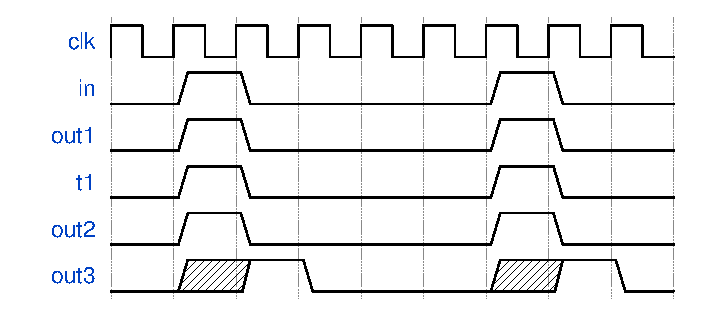
\includegraphics[width=\columnwidth]{figures/wavedrom.eps}%
  \caption{Waveform view showing behavior of RTL design in
  Figure~\ref{figure:equivalence}} 
\label{fig:waveform}
\end{center}
\end{figure}
%
Techniques such as translation validation~\cite{DBLP:conf/tacas/PnueliSS98}  
that check the consistency between an RTL and software is a different problem 
and beyond the scope of this work.
%
%While we do not have a formal proof of equivalence between the Verilog RTL and the 
However, experiments have shown that for 
property verification, valid safety properties are proven to be $k$-inductive for 
the same unwind depth $k$ in the RTL and the software netlist design.  Conversely, 
for unsafe designs, a bug is found in the same unwind depth for both the designs.
             % Equivalence of Hardware and Software
\section{Proposed Verification Tool Flow}
%
\begin{figure}[t]
\centering
\vspace*{0.3cm}
\scalebox{.55}{\import{figures/}{new_flow.pspdftex}}
\caption{Tool flow for hardware property verification\label{fig:toolflow}}
\end{figure}
%
%===============================================================================
%\para{Software Verifiers at the heart of Hardware Verification}
%===============================================================================
%
Figure~\ref{fig:toolflow} shows the tool flow for hardware RTL 
verification at various levels -- 
\emph{bit-level}, \emph{word-level}, and \emph{software netlist-level}.  
The bottom flow of figure~\ref{fig:toolflow} shows the bit-level 
verification flow using \ABC.
\ABC does not support Verilog, so we use an open-source synthesis tool,
\yosys\footnote{http://www.clifford.at/yosys/} to translate Verilog
RTL to BLIF or AIGER, which is then passed to \ABC for verification. 
Given a design in Verilog RTL, \yosys bit-blasts it into a bit-level netlist 
along with the property and the resultant netlist is expressed in And-Inverter 
Graph.  The AIG is represented in AIGER format which is one of the standard 
and most prevelant format used by majority of verification tools.


Whereas, the middle flow of figure~\ref{fig:toolflow} shows the 
word-level verification using the tool 
\ebmc~\footnote{\scriptsize{www.cprover.org/hardware/ebmc}}. 
\ebmc supports IEEE 1364.1 Verilog 2005, and synthesize it to a bit-level 
netlist represented in AIGER or a word-level netlist represented in 
SMT-LIB2 format.  The top flow of figure~\ref{fig:toolflow} shows a
verification flow that synthesize a software netlist from RTL using 
the tool \emph{v2c}.  A wide range of representative software 
verification techniques are applied to determine the safety of the
software netlist models. In particular, we use $k$-induction~\cite{SSS00}
(implemented in the tools CBMC~\cite{cbmc.tacas:2004} and
2LS~\cite{kiki}), interpolation
(CPAChecker~\cite{DBLP:conf/cav/BeyerK11}, IMPARA~\cite{impara}
implementing the IMPACT algorithm~\cite{ken}), abstract interpretation
(Ast{\'r}ee~\cite{DBLP:conf/esop/CousotCFMMMR05}), IC3/PDR
(SeaHorn~\cite{DBLP:conf/cav/GurfinkelKKN15}) and automata-based 
trace abstraction (UltimateAutomizer~\cite{DBLP:conf/tacas/HeizmannDGLMSP16}).
%
%===============================================================================
\section{Experimental Results}
%===============================================================================
In this section, we report experimental results for \emph{unbounded} safety 
verification of hardware RTL.  Our experimental contributions are two folds.
%
\begin{enumerate}
  \item Compare off-the-shelf formal verification tools for RTL verification at 
    \emph{bit-level}, \emph{word-level}, and \emph{software netlist level}.  
    To this end, we compare state-of-the-art hardware model checking tools, such as 
    \emph{ABC 1.01} (winner of HWMCC'15) and 
    \ebmcv~\footnote{\scriptsize{www.cprover.org/hardware/ebmc}}, 
    with various software analyzers from SV-COMP 2016, such as 
    \emph{UltimateAutomizer 3292eade} (winner of SV-COMP'16), 
    \emph{CPAChecker 1.4}, 
    \emph{SeaHorn (revision 07666c810d)}, \emph{2LS 0.3.4}, 
    and a commercial abstract 
    interpretation based tool, \emph{Astr{\'e}e}.  
  
 \item  Compare various unbounded verification engines such as $k$-induction, 
    Interpolation, IC3/PDR and Abstraction Interpretation that are employed by 
    verification tools from hardware and software domains.
\end{enumerate}
%
Our experiments were performed on an Intel Xeon machine running at
3.07\,GHz.  We restricted the resources to 5 hours and 32\,GB RAM per
benchmark.  All our benchmarks in Verilog, software netlist models in 
ANSI-C, scripts for running \yosys, \ABC, \ebmcv, and other software 
verification tools are uploaded to a publicly accessible archive website.
\footnote{\scriptsize{http://www.cprover.org/hardware/tcad/}}
%
%===============================================================================
\para{Benchmarks}
%===============================================================================
%
We verified a total of 35 circuits given in Verilog RTL.  Out of 35, 27 
are \emph{safe} benchmarks and 8 are \emph{unsafe}.  The benchmarks in 
our paper are derived from real world hardware benchmark suites, including 
VIS Verilog models, the Texas-97 Benchmark suite, and opencores.org. We synthesize 
each benchmarks into three different netlist formats -- AIGER, SMT-LIB2, ANSI-C.
We classify our benchmarks into two different classes -- data-path intensive
circuits, including Huffman encoder/decoder and a Digital Audio
Input-Output chip (DAIO); and control-intensive designs,
including a non-pipelined 3-stage processor, a Read-Copy-update
mutual exclusion protocol, a FIFO controller, a buffer allocation model,
and an instruction queue controller.   
%
%-------------------------------------------------------------------------------
\para{Properties}
%-------------------------------------------------------------------------------
%
The safety properties are specified as System Verilog assertions (SVA).
The properties are instrumented as assertions in the software netlist. 
Our tool support fragment of SVA properties. Below, we present
an example of property monitor in software netlist corresponding 
to the concurrent assertions in SVA.  Let us consider verification 
of the following properties of Vending machine and Huffman 
encoder/decoder design. Figure~\ref{figure:prop1} and 
Figure~\ref{figure:prop2} shows the SVA property in the left and 
the corresponding monitor for the software netlist in the right. \\
$Assert\_1$: {\em The balance is never negative and never reaches 15.} 
\vspace{-3mm}
\begin{figure}[htbp]
\scriptsize
\begin{tabular}{l|l}
\hline
SVA & Monitor (in C)
\\
\hline
\begin{lstlisting}[mathescape=true,language=Verilog]
p1: assert property 
 (@(posedge clk) 
 vending.total[3]==0 && 
 !(vending.total[4:0]==15)); 
\end{lstlisting}
&
\begin{lstlisting}[mathescape=true,language=C]
int monitor_p1() {
 assert((((vending.total 
 >> 3) & 0x1) == 0) 
 && !(vending.total 
 & 0x1F == 15));
 return 1;
}
\end{lstlisting} \\
\hline
\end{tabular}
\caption{Modeling concurrent assertions in SVA as monitor in software netlist}
\label{figure:prop1}
\end{figure}
%

$Assert\_2$: {\em When a new transmission begins, the decoder is ready in the next clock.} 
\begin{figure}[htbp]
\scriptsize
\begin{tabular}{l|l}
\hline
SVA & Monitor (in C)
\\
\hline
\begin{lstlisting}[mathescape=true,language=Verilog]
p2: assert property 
 (@(posedge clk) 
 encoder.shiftreg[9:1] 
 == 1 |-> ##1 
 decoder.leaf == 1);
\end{lstlisting}
&
\begin{lstlisting}[mathescape=true,language=C]
int monitor_p2() {
 if(((encoder.shiftreg >> 1) 
 & 0x1FF) == 1) {
  check_consequent = 1;
  // call to top level 
  // module of design
  huffman(clk,addr);  
  if(check_consequent == 1) 
    assert(decoder.leaf == 1);
 }
}
\end{lstlisting} \\
\hline
\end{tabular}
\caption{Modeling temporal properties in SVA as monitor in software netlist}
\label{figure:prop2}
\end{figure}
%
%-------------------------------------------------------------------------------
\para{Discussion}
%-------------------------------------------------------------------------------
We classify the analysis results into two categories -- 1) \emph{precise} tools 
that do not use any abstraction and performs precise reasoning using SAT/SMT solvers 
(in section~\ref{precise}), and \emph{abstraction} based tools that performs 
approximate analysis without using SAT/SMT solvers (in section~\ref{abstraction}). 
%
\subsection{Analysis Using Precise tools}~\label{precise}
%
Figures~\ref{fig:kind}--\ref{fig:hybrid} report the comparison of various unbounded 
verification techniques employed by verification tools at bit-level, word-level, 
and software-level.  The plots in these figures reports the runtimes of~12 
representative circuits which are most difficult to solve out of a total 35 
circuits.  Note that \ABC does not implement word-level verification flow, 
so we perform word-level verification using our in-house tool \ebmc.
Figures~\ref{fig:kind}--\ref{fig:hybrid} reports the best runtimes 
among the bit-level and word-level hardware verification tools.  
%
We categorize the unbounded approaches into three classes:
\begin{compactitem}
\item $k$-induction (Figure~\ref{fig:kind})
\item interpolation (Figure~\ref{fig:impact}), and 
\item PDR together with other hybrid techniques (Figure~\ref{fig:hybrid}).  
\end{compactitem}
By hybrid techniques, we refer to predicate
abstraction as implemented in \emph{CPAChecker} and a combination of
$k$-induction, BMC and abstract interpretation as implemented in
\emph{2LS}~\cite{kiki}.  On the $x$-axis is the analysis time in
seconds and on the $y$-axis we list the benchmarks. The vertical red lines on
the right-hand side of the diagrams show timeouts, out of memory,
inconclusive (unknown) results, errors (crashes), and wrong results
(tool bugs) reported by the tools. The tools can be distinguished 
by the size of the circles as well as by colour. 

\para{Analysis using $k$-induction} For safe benchmarks, the results
for bit-level, word-level verifiers and software verifiers are
comparable when the properties are 1-inductive or 2-step inductive.
However, for complex safety properties, \ABC and other abstraction
based software analyzers either timeout or took a long time to
terminate.  We investigated the reason for higher verification times
for some safe benchmarks, such as the FIFO controller, the RCU, and Buffer 
Allocation.  We observe that the properties are not $k$-inductive for
sufficiently large values of $k$, e.g.\ (k=1000) and thus tools based
on $k$-induction either timeout or took long time to
compute the inductive invariant sufficient to prove the property. For
the unsafe benchmarks, for example DAIO and the traffic light controller, where
the bugs are manifested only at 64 and 65 clock cycles respectively,
the verification times using \ABC and \ebmc's $k$-induction engine 
are comparable to \cbmcv and \textsc{2LS}. Figure~\ref{fig:kind} 
reports the time taken by the $k$-induction engine in 
\ABC, \ebmcv, \cbmcv and \textsc{2LS}.  We did not report
the time for \emph{CPAChecker} since the results suggest that 
its $k$-induction engine is not as mature yet. 

\para{Analysis using Interpolation} Figure~\ref{fig:impact} reports
the time taken by the interpolation engine in \ABC, \textsc{IMPARA}
and \emph{CPAChecker}. \ABC is the fastest in 9 out of 12
designs. However, it timed out on three complex benchmarks, RCU, FIFO
and BufAl, whereas the software interpolation tool, \textsc{IMPARA},
which implements IMPACT algorithm solved three instances out of which
one is the complex FIFO design; yet \textsc{IMPARA} either timed out or
ran out of memory for the remaining designs.  \emph{CPAChecker} solved
5 out of 12 cases.  None of the interpolation engines was able to
prove RCU and BufAl.

\para{Analysis using Hybrid techniques} Figure~\ref{fig:hybrid}
reports the time taken by the IC3/PDR engine in \ABC, \emph{SeaHorn}
and other hybrid techniques as implemented in \emph{CPAChecker} and
\textsc{2LS}. \ABC~is the clear winner here; it is the only tool that
proves the FIFO and BufAl benchmarks safe within the given 5h timeout.
\emph{SeaHorn}'s PDR engine solves half of the benchmarks, but
produces false negatives on the other half due to limited support for
bitvectors. \textsc{2LS} successfully solved 8 benchmarks and times 
out on four benchmarks.  \emph{CPAChecker}'s predicate abstraction reliably
solves 7 benchmarks, but timed out on two benchmarks and reports three
wrong results. Note that none of the tools was able to prove RCU.

The bit-level hardware tools performs better than word-level hardware 
verification for our benchmarks.  So, we only report the bit-level results 
obtained using \ABC in Figures~\ref{fig:kind}--\ref{fig:hybrid}.


%We do not report the results using Astr{\'e}e since it requires manual
%directives for data and control partitioning to avoid imprecision;
%nonetheless it generates many false alarms for safe benchmarks.

%
%%%%%%%%%%%%%%%%%%%%%%%%%%%%%%%%%%%%%%%%%%%%%%%%%%%%%%%%%%%%%%%%%%%%%%%%%%%%%%%%
\begin{figure}
%\scalebox{0.9}{
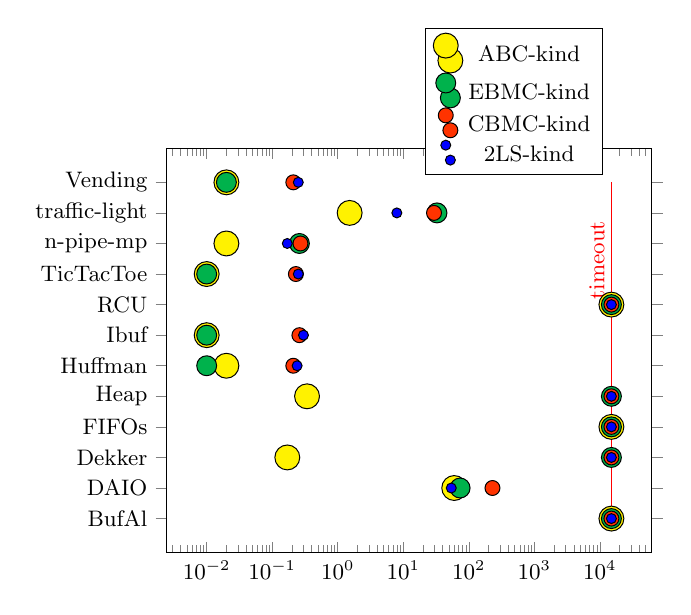
\begin{tikzpicture}[scale=0.9]
\small
\pgfplotstableread{
Benchmark	ABC-kind	EBMC-kind	CBMC-kind	2LS-kind
BufAl	15000	15000	15000	15000
DAIO	59.92	73.62	229.72	54
Dekker	0.17	15000	15000	15000
FIFOs	15000	15000	15000	15000
Heap	0.34	15000	15000	15000
Huffman	0.02	0.01	0.21	0.24
Ibuf	0.01	0.01	0.26	0.3
RCU	15000	15000	15000	15000
TicTacToe	0.01	0.01	0.23	0.25
n-pipe-mp	0.02	0.26	0.27	0.17
traffic-light	1.52	32.67	29.46	7.98
Vending	0.02	0.02	0.21	0.25
}\datatable

\begin{axis}[
    xbar, xmode=log,
    xmin=0,         
    ytick=data,    
    yticklabels from table={\datatable}{Benchmark},  
    legend style={at={(0.9,1.3)}},
]
\addplot [mark size=5pt,only marks, fill=yellow] table [x={ABC-kind}, y expr=\coordindex] {\datatable};    
\addplot [mark size=4pt,only marks, fill=green!70!blue]table [x={EBMC-kind}, y expr=\coordindex] {\datatable};
\addplot [mark size=3pt,only marks, fill=red!80!yellow] table [x={CBMC-kind}, y expr=\coordindex] {\datatable};
\addplot [mark size=2pt,only marks, fill=blue] table [x={2LS-kind}, y expr=\coordindex] {\datatable};
\addplot [red,sharp plot] coordinates{(15000,0) (15000,11)}
          node [left,rotate=90] at (axis cs:9000,10) {timeout};
\legend{{ABC-kind},{EBMC-kind},{CBMC-kind},{2LS-kind}}
\end{axis}
\end{tikzpicture}
%}
\caption{\label{fig:kind}
Comparison of $k$-induction tools
}
\end{figure}
%%%%%%%%%%%%%%%%%%%%%%%%%%%%%%%%%%%%%%%%%%%%%%%%%%%%%%%%%%%%%%%%%%%%%%%%%%%%%%%%

%%%%%%%%%%%%%%%%%%%%%%%%%%%%%%%%%%%%%%%%%%%%%%%%%%%%%%%%%%%%%%%%%%%%%%%%%%%%%%%%
\begin{figure}
%\scalebox{0.9}{
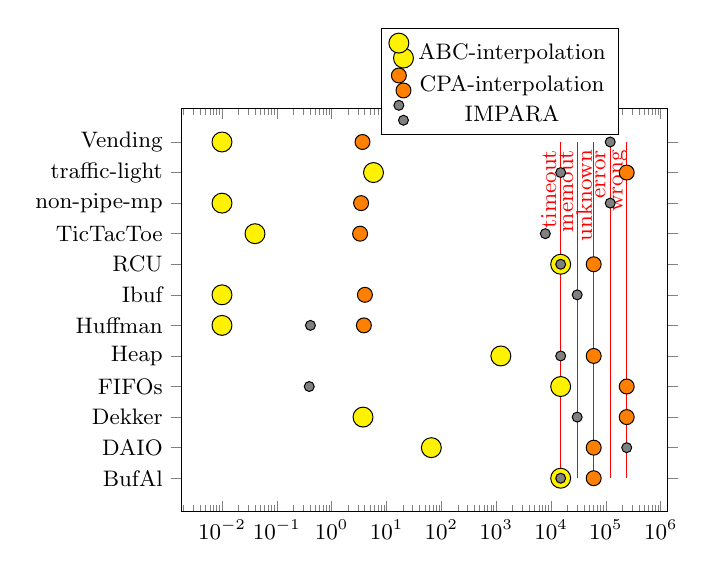
\begin{tikzpicture}[scale=0.9]
\small
\pgfplotstableread{
Benchmark	ABC-interpolation	CPA-interpolation	IMPARA-interpolation
BufAl	15000	60000	15000
DAIO	65.74	60000	240000
Dekker	3.73	240000	30000
FIFOs	15000	240000	0.39
Heap	1215.79	60000	15000
Huffman	0.01	3.87	0.41
Ibuf	0.01	4.04	30000
RCU	15000	60000	15000
TicTacToe	0.04	3.3	7870
non-pipe-mp	0.01	3.44	120000
traffic-light	5.79	240000	15000
Vending	0.01	3.65	120000
}\datatable

\begin{axis}[
    xbar, xmode=log,
    xmin=0,         
    ytick=data,    
    yticklabels from table={\datatable}{Benchmark},  
    legend style={at={(0.9,1.2)}},
]
\addplot [mark size=4pt,only marks, fill=yellow] table [x={ABC-interpolation}, y expr=\coordindex] {\datatable};    
\addplot [mark size=3pt,only marks, fill=orange]table [x={CPA-interpolation}, y expr=\coordindex] {\datatable};
\addplot [mark size=2pt,only marks, fill=gray] table [x={IMPARA-interpolation}, y expr=\coordindex] {\datatable};
\addplot [red,sharp plot] coordinates{(15000,0) (15000,11)}
          node [left,rotate=90] at (axis cs:9000,11) {timeout};
\addplot [red,sharp plot] coordinates{(30000,0) (30000,11)}
          node [left,rotate=90] at (axis cs:19000,11) {memout};
\addplot [red,sharp plot] coordinates{(60000,0) (60000,11)}
          node [left,rotate=90] at (axis cs:40000,11) {unknown};
\addplot [red,sharp plot] coordinates{(120000,0) (120000,11)}
          node [left,rotate=90] at (axis cs:80000,11) {error};
\addplot [red,sharp plot] coordinates{(240000,0) (240000,11)}
          node [left,rotate=90] at (axis cs:180000,11) {wrong};
\legend{{ABC-interpolation},{CPA-interpolation},{IMPARA}}
\end{axis}
\end{tikzpicture}
%}
\caption{\label{fig:impact}
Comparison of interpolation-based tools
}
\end{figure}
%%%%%%%%%%%%%%%%%%%%%%%%%%%%%%%%%%%%%%%%%%%%%%%%%%%%%%%%%%%%%%%%%%%%%%%%%%%%%%%%

%%%%%%%%%%%%%%%%%%%%%%%%%%%%%%%%%%%%%%%%%%%%%%%%%%%%%%%%%%%%%%%%%%%%%%%%%%%%%%%%
\begin{figure}
%\scalebox{0.9}{
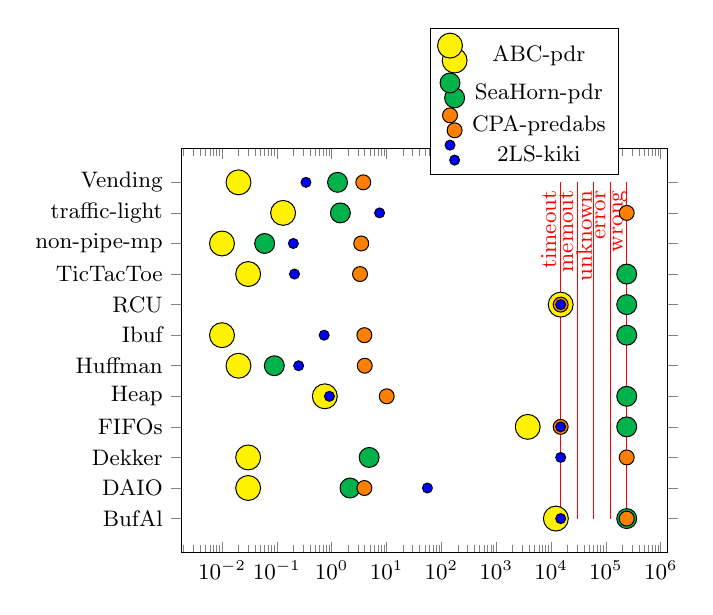
\begin{tikzpicture}[scale=0.9]
\small
\pgfplotstableread{
Benchmark	ABC-pdr	SeaHorn-pdr	CPA-predabs	2LS-kiki
BufAl	12250.5	240000	240000	15000
DAIO	0.03	2.16	3.95	55.72
Dekker	0.03	4.83	240000	15000
FIFOs	3759.75	240000	15000	15000
Heap	0.75	240000	10.09	0.91
Huffman	0.02	0.09	4.01	0.25
Ibuf	0.01	240000	3.95	0.73
RCU	15000	240000	15000	15000
TicTacToe	0.03	240000	3.29	0.21
non-pipe-mp	0.01	0.06	3.46	0.20
traffic-light	0.13	1.44	240000	7.48
Vending	0.02	1.28	3.77	0.34
}\datatable

\begin{axis}[
    xbar, xmode=log,
    xmin=0,         
    ytick=data,    
    yticklabels from table={\datatable}{Benchmark},  
    legend style={at={(0.9,1.3)}},
]
\addplot [mark size=5pt,only marks, fill=yellow] table [x={ABC-pdr}, y expr=\coordindex] {\datatable};    
\addplot [mark size=4pt,only marks, fill=green!70!blue]table [x={SeaHorn-pdr}, y expr=\coordindex] {\datatable};
\addplot [mark size=3pt,only marks, fill=orange] table [x={CPA-predabs}, y expr=\coordindex] {\datatable};
\addplot [mark size=2pt,only marks, fill=blue] table [x={2LS-kiki}, y expr=\coordindex] {\datatable};
\addplot [red,sharp plot] coordinates{(15000,0) (15000,11)}
          node [left,rotate=90] at (axis cs:9000,11) {timeout};
\addplot [red,sharp plot] coordinates{(30000,0) (30000,11)}
          node [left,rotate=90] at (axis cs:19000,11) {memout};
\addplot [red,sharp plot] coordinates{(60000,0) (60000,11)}
          node [left,rotate=90] at (axis cs:40000,11) {unknown};
\addplot [red,sharp plot] coordinates{(120000,0) (120000,11)}
          node [left,rotate=90] at (axis cs:80000,11) {error};
\addplot [red,sharp plot] coordinates{(240000,0) (240000,11)}
          node [left,rotate=90] at (axis cs:180000,11) {wrong};
\legend{{ABC-pdr},{SeaHorn-pdr},{CPA-predabs},{2LS-kiki}}
\end{axis}
\end{tikzpicture}
%}
\caption{\label{fig:hybrid}
Comparison of hybrid techniques
}
\end{figure}
%%%%%%%%%%%%%%%%%%% Plot runtimes %%%%%%%%%%%%%%%%%%%%%%%
\begin{figure}[t]
  \centering
  \begin{tikzpicture}[scale=0.60]

\pgfplotscreateplotcyclelist{markstyles}{%
solid, every mark/.append style={solid, fill=white}, mark=square*, mark size=2.5\\%
solid, every mark/.append style={solid, blue}, mark=triangle*,mark size=2.5\\%
solid, every mark/.append style={solid, fill=black}, mark=otimes*,, mark
    size=2.5\\%
}
    
 	%axis
  \begin{axis}[
    width=\linewidth,
    xlabel={Benchmark Number},
    ylabel={Time (seconds)},
    domain = 1:40,
    xmin=1, xmax=34,
    ymin=0, ymax=200,
    %ytick={0,20,...,200},
    xtick={1,5,10,...,34},
    width=15cm, height= 7cm,
    ymode = log,
    %log basis x={2},
    %xticklabel=\pgfmathparse{2^\tick}\pgfmathprintnumber{\pgfmathresult},
    legend pos = north west,
    grid = major,
    major grid style={line width=.2pt,draw=gray!50},
    cycle list name=markstyles
  ]
	
  %plots
  %\addplot table [only marks, y=Time, x=Benchmarks]{plotdata/cbmc.dat};
	%\addlegendentry{CBMC}
  
  \addplot table [only marks, y=Time, x=Benchmark]{plotdata/ultimate.dat};
  \addlegendentry{UltimateAutomizer}
  
  \addplot table [only marks, y=Time, x=Benchmark]{plotdata/astree.dat};
  \addlegendentry{Astr{\'e}e}
	
  \end{axis}  
\end{tikzpicture}
\caption{\label{fig:runtimes}
  Runtime Comparison between UltimateAutomizer and Astr{\'e}e}
\end{figure}

%%%%%%%%%%%%%%%%%%%%%%%%%%%%%%%%%%%%%%%%%%%%%%%%%%%%%%%%%
\subsection{Analysis Using Abstraction based tools}~\label{abstraction}
%
Figure~\ref{fig:runtimes} gives the runtime comparsion between ABC, UltimateAutomizer 
and Astr{\'e}e.  Both UltimateAutomizer and Astr{\'e}e operate on an overapproximate 
abstraction of the concrete program.  


\ABC proved a total of 31 benchmarks and timed out for 4 benchmarks. 
The results in figure~\ref{fig:runtimes} are obtained using ABC PDR engine. 
The runtimes of Astr{\'e}e are very close to ABC for most benchmarks. Astr{\'e}e 
was faster than \ABC in 3 cases.  However, Astr{\'e}e reported a total of 
7 false alarm out of 35 benchmarks, marked as timeout in blue traiangles 
in figure~\ref{fig:runtimes}.  
We investigate the reason for the false alarm and observe 
that the bit manipulating nature of these programs prevent Astr{\'e}e from 
inferring the necessary invariants required to prove the property using the 
existing set of abstract domains.  Whereas, UltimateAutomizer timed out in~14 
out of 30 benchmarks. For safe benchmarks that are hard to proof, UltimateAutomizer 
was able to infer the necessary invariants required to prove the property within 
feasible time, as shown by square boxes between benchmark number 25 to 35, while 
Astr{\'e}e was too imprecise to prove the property for these benchmarks. Astr{\'e}e 
performed better than UltimateAutomizer for the unsafe benchmarks.  Astr{\'e}e 
reported bugs in all 8 unsafe benchmarks within the time limit. 


We now discuss the analysis using these abstraction based tools.

\para{Abstract Interpretation of RTL}
%
One of the benefits of the proposed tool flow in this paper is that the 
synthesis of RTL to software netlist enables the application of techniques 
such as abstract interpretation. Abstract Interpretation~\cite{Cousot92,CC79} 
is a theory of sound approximation of program semantics based on lattice 
structures. Static analysis using abstract interpretation is widely used 
to verify properties of safety-critical systems. 


Astr{\'e}e~\cite{DBLP:conf/esop/CousotCFMMMR05} is a commercial abstract 
interpretation tool developed by AbsInt~\footnote{https://www.absint.com/}.  
It is primarily used for static analysis of safety-critical softwares 
such as avionics software~\cite{DBLP:journals/corr/abs-cs-0701193}.
Astr{\'e}e employs numeric abstract domains, such as intervals that  
abstract variable values as ranges, as well as relational domains that  
infer linear and non-linear relationships between variables. These abstractions are  
well-suited for programs performing integer and float arithmetic, but  
less so for bit-level Boolean operators, bit-shifts, and bitfields  
packing several values in words.  The non-linear abstract domains in 
Astr{\'e}e such as quadratic and exponential functions are mostly useful 
for aerospace applications~\cite{DBLP:journals/ftpl/BertraneCCFMMR15}.  
Moreover, Astr{\'e}e features BDD-based abstract 
domains~\cite{bdd-domain} that can represent non-convex invariants, 
but they are currently limited to Boolean variables and cannot perform  
bit-blasting on integer variables.  For bit manipulating programs 
generated by \textsc{v2c}, Astr{\'e}e uses default abstract domains 
for integer values such as interval domain, octagon domain, integer 
congruences, integer bitfields, and finite sets (of possible values).


When Astr{\'e}e encounters an \texttt{assert}, it first checks whether 
there are some program states that do not satisfy the assertion, and 
then continues the analysis with only the states that satisfy the assertion. 
Indeed, it assumes that the states that do not satisfy the assertion cause 
the program to stop.  A message such as ``Definite assertion failure" appears 
in case there are no states satisfying the assertion at all, hence, the 
instructions following the assertion are never executed.


%%%%%%%%%%%%%%%%%%%%%%%%%%%%%%%%%%%%%%%%%%%%%%%%%%%%%%%%%%%%%%%%%%%%%%%%%%%%%%%%
%\para{Effect of Trace partitioning for Precise analysis in Astr{\'e}e}
%%%%%%%%%%%%%%%%%%%%%%%%%%%%%%%%%%%%%%%%%%%%%%%%%%%%%%%%%%%%%%%%%%%%%%%%%%%%%%%%
%
\para{Handling Imprecision in Astr{\'e}e}
%
Given that many abstract domains can only represent convex  
(non-disjunctive) numeric properties, control-flow joins and loop  
widening are a major cause of precision loss.  Astr{\'e}e partially  
alleviates the problem through BDD-based domains and 
trace-partitioning~\cite{DBLP:journals/toplas/RivalM07}
(providing a level of path-sensitivity). 
To prevent scalability 
 issues, 
 these costly techniques are enabled locally, 
 through automatic heuristics 
or user guidance.  That is, a partitioning initiated inside a function will be merged over before  
returning from the function, so, it's function-local. Sometimes, a  
longer partitioning is useful, but it is not generated by the  
heuristics (although it can be generated by hand).  While standard 
widening can cause lot of precision loss, Astr{\'e}e 
uses more gradual widening and does not losses all precision at  
once.  We employ widening with thresholds, for instance, and also delay  
the widening (independently on each variable).  


With trace partitioning, Astr{\'e}e automatically insert 
\texttt{\_\_ASTREE\_partition\_control} directives according to a set of 
heuristics.  Astr{\'e}e does not partition ``everything" since this would 
be too expensive in practise. Such a high precision is also normally not 
required for a runtime error analysis. Astr{\'e}e normally start with exisitng 
partitioning heuristics and manually add partitioning directives in places 
where false alarms occur due to a loss of precision resulting from merging 
data-flow information of several control-flow paths (traces).
There are two partitioning strategies in Astr{\'e}e - 
1) control-flow partition and 2) partition over all relevant variable values.
Both can be either specified by hand or using automatic  
partitioning or (more likely) a combination of both. Automatic  
partitioning is simply a fast pre-analysis that inserts  
$\_\_ASTREE\_partition$ directives into the Abstract Syntax Tree.

A classic example of control partitioning is to analyze each branch of a 
control-flow path separately so as to prevent joins at the control-flow merge 
point.  An example of variable partitioning is as follows. Consider a variable 
named \texttt{mode} that can assume values between 1 and 5.  A partitioning directive 
\texttt{\_\_ASTREE\_partition\_begin((mode));} tells Astr{\'e}e to keep all 
five traces for all five possible values of mode apart 
until the next merge point (i.e., the end of a function, a loop, a sub-statement 
or a merge directive). This of course requires Astr{\'e}e to know that mode is 
in the range $[1;5]$.


Although one can theoretically get an arbitrary high precision in Astr{\'e}e by 
partitioning such that all relevant (or in the extreme: possible) execution 
paths are considered separately, but that is not feasible in practice considering 
the analysis times. Hence, the trick is to find the ``right" partitioning that 
is as imprecise as possible, but can still prove the property under verification. 
But this is a challenging task.  
%Astr{\'e}e does not collect data about 
%state-space coverage of variables to help user find a good partitioning. 
However, Astr{\'e}e can show the user any variable range and invariants that 
it has computed.  So, the user can use this information to  
add manually more partitioning and re-run the analysis. What Astr{\'e}e lack  
is a way for this information to be used automatically in partitioning  
strategies during the subsequent analyses.  For our benchmarks, 
%I did not have time to 
we inspect all the invariants inferred by Astr{\'e}e and added the 
necessary partitioning.  A few false alarms in Astr{\'e}e is avoided 
using this strategy.  However, this require manual intervention to 
guide the tool to precisely prove a property of the software netlist model.


%Hence, some amount of domain knowledge is required to try different partitioning 
%strategies that might enable the analysis to prove the properties under verification. 
%For our experiments, we ran the analysis using the existing heuristics and manual 
%partitioning on data as well as control that target automatically-generated 
%software netlist obtained from \textsc{v2c} and 
%was sufficient to precisely prove the properties. 


\Omit{
There can be various sources of imprecision in abstract 
interpretation.  Few common sources of imprecision may occur due to   
\emph{control-flow join}, \emph{loop widening} or use of \emph{imprecise abstract domain}.  
We analyzed the structure of software netlist models to detect the potential sources of 
imprecision that may occur during the analysis using Astr{\'e}e.  Recall that the software 
netlist model retains the control structure of the input RTL design.  Hence, if the original 
RTL has loops or conditional branches inside a module, a software netlist also preserves the 
similar control structure.   
}

\para{Soundness of Astr{\'e}e}
%
Astr{\'e}e is sound, that is, it does not miss any genuine error. 
However, it errs for the safe benchmarks, sometimes too much. Hence, Astr{\'e}e 
may report more false positives than other tools. However, Astr{\'e}e 
found genuine bugs in all 8 unsafe benchmarks.
%(doing otherwise would be a bug in Astrée). 
In general, a sound tool is useful for validation, less so for 
bug-finding.


\Omit{Standard Static Analysis is Imprecise, but can we do better than bit
blasting ? 

\para{Idea} Partition the traces so that we can prove correctness for each partition.
\para{Solution} To be effecient, we want partitions that are just precise
enough. 
}
\Omit{Best HW runtime versus Best Software runtimes}

\subsection{Summary of the results} 
%
We summarize the results obtained from the precise and abstraction based 
software verification tools for verifying software netlist models synthesized
from a RTL circuit.  

\para{Analysis using Precise SAT/SMT based Software Tools}
%
Though the invariant inference techniques employed by precise software 
analyzers such as \emph{CPAChecker} and \emph{2LS} have never
been optimized for hardware analysis, but the results in this paper
show that these tools are within one order of magnitude compared to
hardware model checkers for detecting bugs or proving safety for some
of the software netlist models.  However, running precise SAT/SMT 
based sotware verification tools on software netlists exhibits many 
%tool bugs (marked as ``wrong'' in Figure).
%We investigated the reason for large number of 
timeouts, wrong results and errors.  We observed that software netlists 
heavily use bit-level operations and thus bit-precise reasoning ability 
is necessary for the underlying verification engine. However, bit-level operations 
are less prevalent in conventional software and hence less tested in software 
analysis tools.  \rmcmt{We reported the tool bugs to the authors of these tools.} 


\para{Analysis using Abstraction based Software Tools}
%
The abstraction based tools such as Ultimate Automizer and Astr{\'e}e 
performed better than the precise SAT/SMT based tools on the software 
netlist models.  Though Astr{\'e}e require manual intervention 
to select the right set of partitions of program traces in order to do 
precise analysis, the verification runtimes are comparable to \ABC for 
most of the benchmarks.  However, Astr{\'e}e often use numerical 
abstractions, which are likely to lose important bit-precise information.  
As a consequence, many inductive invariants required by the bit-manipulating 
benchmarks cannot be represented, and so not inferred, using current abstractions 
in Astr{\'e}e.  An abstract domain for this purpose must keep 
precise relations between the bits of an integer (possibly some 
form of BDD on the bits of the variable).  Astr{\'e}e has already been 
refined for avionics and space software by adding few domain-specific 
abstract domains which were very effective in removing some classes of 
false alarms~\cite{DBLP:journals/ftpl/BertraneCCFMMR15}.  We thus believe 
that there is scope here for new abstract domains targeting hardware 
designs while still remaining within the scope of traditional abstract 
interpreter. 
%
%that implement abstract interpretation using
%abstract domains developed specifically for this task, e.g.~by
%applying abstract conflict driven learning~\cite{dhk2013-popl}.  
\Omit{
%-------------------------------------------------------------------------------
\para{Limitations of the Result}
%-------------------------------------------------------------------------------
Due to lack or absence of Verilog support in other open-source tools that
participate in the HWMCC competition, like \emph{PdTrav}, \emph{IIMC} and 
\emph{V3}, we could not run these tools on our benchmark suite. 
}

\Omit{
The range of software verification techniques is vast; this paper can
thus only be an initial step.  We will evaluate further software
verification techniques and their application to hardware property
checking and co-verification workloads as future work.
}
              % Experiments.
\section{Related Work}~\label{related_work}
%
%%%%%%%%%%%%%%%%%%%%%%%%%%%%%%%%%%%%%%%%%%%%%%
%      Bit-level Verification Literature
%%%%%%%%%%%%%%%%%%%%%%%%%%%%%%%%%%%%%%%%%%%%%%

%%%%%%%%%%%%%%%%%%%%%%%%%%%%%%%%%%%%%%%%%%%%%%
%     Word-level Verification Literature
%%%%%%%%%%%%%%%%%%%%%%%%%%%%%%%%%%%%%%%%%%%%%%

%%%%%%%%%%%%%%%%%%%%%%%%%%%%%%%%%%%%%%%%%%%%%%
%      Software verification Literature
%%%%%%%%%%%%%%%%%%%%%%%%%%%%%%%%%%%%%%%%%%%%%%

The technology transfer between the hardware and software verification community 
over the past two decades have demonstrated significant drive in development of 
new verification algorithms in either field. 
% 
In 1986, Clarke et al.~\cite{clarke86} proposed model checking for finite state 
concurrent systems. Later, McMillan et. al.~\cite{mcmillan96} introduced symbolic 
model checking in 1996.  Biere et al.~\cite{tacas99} introduced symbolic model 
checking without BDDs in 1999.
%
Graf et al.~\cite{cav97} proposed a technique based on predicate abstraction.
Later, Clarke et. al.~\cite{cav2000} used Counterexample guided Abstraction Refinement 
(CEGAR) in SMV tool for verifying Fujitsu IP core.  
Kroening et. al.~\cite{DBLP:conf/tacas/JainKSC07} used CEGAR to 
verify hardware designs written in Verilog RTL.  Subsequently, predicate 
abstraction is used for verifying device drivers in C program by Ball et al.~\cite{pldi01}.  
This lead to the SLAM project by Ball et. al.~\cite{popl02} in 2002.
%
In 2000, St$\mathring{\text{a}}$lmarck et al.~\cite{fmcad2000} introduced a technique 
to check safety properties using Induction and SAT solver.  Subsequnetly, induction 
based approaches are used for automatic analysis of scratch-pad memory code for heterogeneous
multicore processors by Donaldson et. al.~\cite{tacas10}, 2010 and for software 
verification using k-induction by Donaldson et al.~\cite{sas2011} in 2011.
% 
In 2003, McMillan et al.~\cite{cav03} introduced Interpolation and SAT-based model 
checking for verifying commercial microprocessor. Subsequently, Intrpolation is used 
for software verification by McMillan et. al.~\cite{cav06} in 2006 and by 
Kroening et al.~\cite{DBLP:conf/cav/KroeningW11}, in 2011.
%
In 2007, Bradley et. al.~\cite{fmcad07} introduced safety checking by inductive 
generalizations of counterexample to induction, a technique commonly known 
as IC3. Subsequnetly, IC3 is used for software model checking by 
Cimatti et al.~\cite{cav12ic3} in 2012.
%
Thus, techniques like predicate abstraction, 
IC3 or Property Directed Reachability (PDR), $k$-induction, and 
interpolation-based approaches have all made their way from the hardware 
to the software domain; but path-wise symbolic execution and abstract 
interpretation have been primarily used for software verification.
%
A survey of bounded and unbounded SAT-based hardware model checking techniques 
is presented in~\cite{DBLP:conf/charme/AmlaDKKM05}.
%

\Omit{
A survey of bounded and unbounded SAT-based hardware model checking techniques 
is presented in~\cite{charme05}.
Table~\ref{timeline} provides a summary of technology transfer between the 
hardware verification community and software verification community over the past 
two decades.  The table provides the reference to the very first technique proposed 
in the literature in either community but there are subsequent works that
follows up from these.  For example, techniques like predicate abstraction, 
IC3 or Property Directed Reachability (PDR), $k$-induction, and 
interpolation-based approaches have all made their way from the hardware 
to the software domain; but path-wise symbolic execution and abstract 
interpretation have been primarily used for software verification.
%
\begin{table}[]
\centering
\scriptsize
\caption{Technology transfer between the Hardware and Software Verification Community}
\label{timeline}
\begin{tabular}{p{0.2\textwidth}|p{0.2\textwidth}}
\toprule
  Hardware Verification & Software Verification \\
  \midrule
  \begin{itemize}
  \item Symbolic Model Checking without BDDs 
    by Biere et. al.~\cite{tacas99}, 1999
\end{itemize}
 & 
 \begin{itemize}
  \item Model Checking for finite state concurrent systems by Clarke et
    al.~\cite{clarke86}, 1986
  \item Symbolic Model Checking by McMillan et. al.~\cite{mcmillan96}, 1996
\end{itemize} \\ \hline

 \begin{itemize}
 \item Predicate Abstraction by Graf et. al.~\cite{cav97}, 1997
 \item CEGAR in SMV for verifying Fujitsu IP core by Clarke et.
   al.~\cite{cav2000}, 2000 
 %\item CEGAR for Verilog by Kroening et. al.~\cite{tacas07}, 2007
 \end{itemize}
  &
  \begin{itemize}
    \item Predicate Abstraction for C program by Ball et. al.~\cite{pldi01},
      2001
    \item SLAM project by Ball et. al.~\cite{popl02}, 2002
  \end{itemize} \\ \hline
 
  \begin{itemize}
    \item Checking safety properties using Induction and SAT solver by
      St$\mathring{\text{a}}$lmarck et. al.~\cite{fmcad2000}, 2000
   \end{itemize}
   & 
   \begin{itemize}
     \item Automatic analysis of scratch-pad memory code for heterogeneous
       multicore processors by Donaldson et. al.~\cite{tacas10}, 2010
     \item Software verification using k-induction by Donaldson et.
       al.~\cite{sas2011}, 2011
   \end{itemize} \\ \hline
   
   \begin{itemize}
     \item Interpolation and SAT-based model checking for verifying commercial
       microprocessor by McMillan et. al.~\cite{cav03}, 2003
   \end{itemize}
   & 
   \begin{itemize}
     \item Lazy abstraction with interpolants by McMillan et. al.~\cite{cav06}, 2006
     \item Interpolation based software verification with Wolverine by Kroening
       et. al.~\cite{cav11}, 2011
   \end{itemize} \\ \hline
   
   \begin{itemize}
     \item Checking safety by inductive generalizations of counterexample to
       induction by Bradley et. al.~\cite{fmcad07}, 2007
   \end{itemize}
   &
   \begin{itemize}
    \item Software Model Checking via IC3 by Cimatti et. al.~\cite{cav12ic3}, 2012
   \end{itemize} \\ \hline
\bottomrule
\end{tabular}
\end{table}
%
}

\section{Conclusions}\label{sec:concl}
%
Demand for more scalable verification tools is ever growing.  In this paper,
we present an alternative solution for verifying hardware, at the heart of
which is a verifier for software.  To this end, we present a technique to 
synthesize a software netlist from Verilog RTL.  We then use state-of-the-art
software verification tools to verify these software netlist models.  Our 
experimental results present a detailed comparison of various unbounded 
verification algorithms at bit-level, word-level and software level.  Our proposed 
hardware verification flow enables seamless adoption of any advances in software 
verification technology to RTL verification.  We observe that bit-level operations 
are less prevelant in conventional software and hence software analyzers are not 
optimized to reason about bit manipulating software programs.  However, most software 
tools are able to successfully verify RTL circuits and the performance of these tools 
are within an order of magnitude compared to bit-level hardware tools.  Existing abstract 
domains used in abstraction based software tools are insufficient for precise reasoning 
of software netlist models.  This can be addressed by either developing heuristics 
more adapted to the code generated by v2c, or manually annotating the generated code 
to improve the precision of the analysis. In this paper, we follow the later approach 
to obtain the desired results. 
    % Conclusions

% ---------------------------------------------------------------------
% Un-numbered section of acknowledgments
% ---------------------------------------------------------------------

\section*{Acknowledgments}

% ---------------------------------------------------------------------
% Bibliography
% ---------------------------------------------------------------------

\bibliographystyle{IEEEtran}
\bibliography{biblio}

% ---------------------------------------------------------------------
% Biographies of authors.
% ---------------------------------------------------------------------

% \begin{IEEEbiography}{Rajdeep Mukherjee}
% \end{IEEEbiography}

% \begin{IEEEbiography}{Peter Schrammel}
% \end{IEEEbiography}

% \begin{IEEEbiography}{Tom Melham}
% \end{IEEEbiography}

% \begin{IEEEbiography}{Daniel Kroening}
% \end{IEEEbiography}

% \begin{IEEEbiography}{Michael Tautschnig}
% \end{IEEEbiography}

\end{document}


